\documentclass[3p,authoryear,fleqn]{elsarticle}
\journal{NeuroImage (Accepted paper YNIMG13167)}
\usepackage[utf8]{inputenc}
\defcitealias{esteban_useful_2016}{Supplemental Materials}
\usepackage{xifthen}
\newboolean{review}
\setboolean{review}{false}

\usepackage{tikz}
\usepackage[mode=buildnew]{standalone}
\usepackage{gincltex}
\usepackage{glossaries}
\usepackage{booktabs} \usepackage{multirow}

\usepackage{xcolor}
\usepackage{url}
\usepackage[colorlinks=true]{hyperref}
\usepackage{doi}

\usepackage{xspace}
\usepackage{graphicx}
\graphicspath{{YNIMG13167_figures/}}

\usepackage{mathtools}
\usepackage{amsmath}
\usepackage{amssymb}
\usepackage{cancel}
\DeclareMathOperator{\tr}{tr}
\DeclareMathOperator{\argmax}{argmax}
\DeclareMathOperator{\argmin}{argmin}
\DeclareMathOperator{\diag}{diag}
\DeclareMathOperator{\dist}{dist}
\DeclareMathOperator{\const}{Const.}
\providecommand{\e}[1]{\ensuremath{\cdot\text{10}^\text{#1}}}
\providecommand{\mdist}[2]{ \mathcal{D}_{#2}^2(\mathbf{#1}) }
\providecommand{\omegaset}{\ensuremath{\boldsymbol{\Omega}}}
\providecommand{\gammaset}{\ensuremath{\boldsymbol{\Gamma}}}
\providecommand{\regseg}{\emph{regseg}}
\providecommand{\Regseg}{\emph{Regseg}}
\providecommand{\lowb}{\textit{b0}}

\let\oldhat\hat
\renewcommand{\vec}[1]{\mathbf{#1}}

\providecommand{\nvec}[1]{\hat{\mathbf{#1}}}

\providecommand{\isores}[2][]{#2\ensuremath{\times}#2\ensuremath{\times}#2\ifthenelse{\equal{#1}{}}{}{ [#1]}\xspace}

\hyphenation{op-tical net-works semi-conduc-tor an-isot-ropy regis-tra-tion iso-tropic Free-Surfer align-ed pre-sent work-flow data-set data-sets micro-struc-tu-re Ma-drid non-linear de-for-ma-tion
an-iso-tro-pic Stud-holme seg-ment-a-tion re-gis-tra-tion map-ped achiev-ed}

\newacronym{mr}{MR}{magnetic resonance}
\newacronym{mri}{MRI}{magnetic resonance imaging}
\newacronym{dwi}{DWI}{diffusion weighted image}
\newacronym{dmri}{dMRI}{diffusion MRI}
\newacronym{dw}{DW}{diffusion weighted}
\newacronym{dti}{DTI}{diffusion tensor imaging}
\newacronym{t1}{T1w}{T1-weighted}
\newacronym{t2}{T2w}{T2-weighted}
\newacronym{csf}{CSF}{cerebrospinal fluid}
\newacronym{wm}{WM}{white matter}
\newacronym{gm}{GM}{gray matter}
\newacronym{epi}{EPI}{echo-planar imaging}
\newacronym{gre}{GRE}{gradient echo sequence}
\newacronym{fa}{FA}{fractional anisotropy}
\newacronym{md}{MD}{mean diffusivity}
\newacronym{adc}{ADC}{apparent diffusion coefficient}
\newacronym{acwe}{ACWE}{active contours without edges}
\newacronym{adf}{ADF}{active deformation field}
\newacronym{map}{MAP}{maximum a posteriori}
\newacronym{snr}{SNR}{signal-to-noise ratio}
\newacronym{pve}{PVE}{partial volume effect}
\newacronym{roi}{ROI}{region of interest}
\newacronym{mrf}{MRF}{Markov Random Field}
\newacronym{pde}{PDE}{partial differential equation}
\newacronym{swindex}{sWI}{surface warping index}
\newacronym{wi}{WI}{Warping index}
\newacronym{nof}{NoF}{number of fibers}
\newacronym{t2b}{T2B}{T2w-registration based}
\newacronym{fft}{FFT}{fast Fourier transform}
\newacronym{hcp}{HCP}{Human Connectome Project}
\newacronym{pe}{PE}{phase-encoding}
\newacronym{ci}{CI}{confidence interval}
\newacronym[first={tract-based spatial statistics --TBSS--}]{tbss}{TBSS}{tract-based spatial statistics}

\newacronym[first={AMICO \cite[accelerated microstructure imaging via convex optimization,][]{daducci_accelerated_2015}}]{amico}{AMICO}{accelerated microstructure imaging via convex optimization}

\makeglossaries

 
\usepackage[T1]{fontenc}
\usepackage{charter}

\usepackage{array}
\newcolumntype{L}[1]{>{\raggedright\let\newline\\\arraybackslash\hspace{0pt}}m{#1}}

\usepackage{ifpdf}
\usepackage[switch]{lineno}

\ifthenelse{\boolean{review}}
{
  \usepackage[colorinlistoftodos,textsize=tiny, textwidth=1.2cm]{todonotes}
  \colorlet{revcolor}{blue!70}
  \setlength{\marginparwidth}{1.5cm}
  \reversemarginpar
    \newcommand{\revcomment}[2][]{\ifthenelse{\equal{#1}{}}{}{\todo{#1}}  \begingroup \color{revcolor} #2\endgroup}
}
{
  \definecolor{revcolor}{gray}{0.0}
  \newcommand{\todo}[2][]{}
  \newcommand{\revcomment}[2][]{#2}
}

\def\bibsection{\section*{References}}

\begin{document}
\hypersetup{linkcolor=black!60, citecolor=black!60, urlcolor=black!60}
\begin{frontmatter}


\title{Surface-driven registration method for the structure-informed segmentation of diffusion MR images\tnoteref{t1}}
\tnotetext[t1]{Supplemental materials to this work have been submitted to Data in Brief \citep{esteban_useful_2016}.
During the review process, the document is available in doi:\href{http://figshare.com/s/459c26b4ee8211e493b306ec4bbcf141}{10.6084/m9.figshare.1397502}.}

\author[bit,ciber]{Oscar~Esteban\corref{corrauthor}}
\cortext[corrauthor]{Corresponding author}
\ead{phd@oscaresteban.es}
\author[ucla]{Dominique~Zosso}
\author[lts5]{Alessandro~Daducci}
\author[chuv,lts5]{Meritxell~Bach-Cuadra}
\author[bit,ciber]{Mar\'ia-J.~Ledesma-Carbayo}
\author[lts5,chuv]{Jean-Philippe~Thiran}
\author[bit,ciber]{Andres~Santos}


\address[bit]{Biomedical Image Technologies (BIT), ETSI Telecomunicaci\'on, Universidad Polit\'ecnica de Madrid, Madrid, Spain}
\address[ciber]{Centro de Investigaci\'on Biom\'edica en Red en Bioingenier\'ia, Biomateriales y Nanomedicina (CIBER-BBN), Spain}
\address[ucla]{Department of Mathematics, University of California,
Los Angeles (UCLA), Los Angeles, CA, US}
\address[lts5]{Signal Processing Laboratory (LTS5), \'Ecole Polytechnique
F\'ed\'erale de Lausanne (EPFL), Lausanne, Switzerland}
\address[chuv]{Dept. of Radiology, CIBM, University
Hospital Center (CHUV) and University of Lausanne (UNIL), Lausanne, Switzerland}


\begin{abstract}
Current methods for processing \gls*{dmri} to map the connectivity of the human brain
  require precise delineations of anatomical structures.
This requirement has been approached by either segmenting the data in
  native \gls*{dmri} space or mapping the structural information from \gls*{t1} images.
The characteristic features of diffusion data in terms of \acrlong*{snr}, resolution, as well
  as the geometrical distortions caused by the inhomogeneity of magnetic susceptibility
  across tissues hinder both solutions.
Unifying the two approaches, we propose \regseg{}, a surface-to-volume nonlinear
  registration method that segments homogeneous regions within multivariate images by mapping
  a set of nested reference-surfaces.
Accurate surfaces are extracted from a \gls*{t1} image of the subject, using as target image
  the bivariate volume comprehending the \gls*{fa} and the \gls*{adc} maps derived from the
  \gls*{dmri} dataset.
We first verify the accuracy of \regseg{} on a general context using digital phantoms 
  distorted with synthetic and random deformations.
Then we establish an evaluation framework using undistorted \gls*{dmri} data from the \gls*{hcp}
  and realistic deformations derived from 
  the inhomogeneity fieldmap corresponding to each subject.
We analyze the performance of \regseg{} computing the misregistration error of the surfaces estimated
  after being mapped with \regseg{} onto 16 datasets from the \gls*{hcp}.
The distribution of errors shows a 95\% CI of 0.56--0.66 mm, that is below the \gls*{dmri}
  resolution (1.25 mm, isotropic).
Finally, we cross-compare the proposed tool against a nonlinear \lowb{}-to-T2w registration
  method, thereby obtaining a significantly lower misregistration error with \regseg{}.
The accurate mapping of structural information in \gls*{dmri} space 
  is fundamental to increase the reliability of network building
  in connectivity analyses, and to improve the performance of the emerging structure-informed
  techniques for \gls*{dmri} data processing. \end{abstract}


\begin{keyword}
active~surfaces \sep cortical~parcellation \sep diffusion MRI \sep nonlinear~registration \sep segmentation \sep susceptibility~distortion.
\end{keyword}

\end{frontmatter}

\ifthenelse{\boolean{review}}{\linenumbers}{}
\section{Introduction}\label{sec:regseg-intro}
\Acrlong*{dmri} enables the mapping of microstructure \citep{basser_microstructural_1996}
  and connectivity \citep{craddock_imaging_2013} of the human brain \emph{in-vivo}.
It is generally acquired using \gls*{epi} schemes, since they are very fast at
  scanning a large sequence of images called \glspl*{dwi}.
Each \gls*{dwi} is sensitized with a gradient to probe proton diffusion in a certain
  orientation.
Subsequent processing involves describing the local microstructure with one of the available
  models, which range from the early \gls*{dti} proposed by \cite{basser_microstructural_1996}
  to current models such as \gls*{amico}.
The microstructural map is then used to draw the preferential orientations of diffusion
  across the brain using tractography \citep{mori_threedimensional_1999}.
Finally, a graph representing the corresponding structural network is built using
  the regions of a cortical parcellation as nodes and the fiber paths found by
  tractography as edges \citep{hagmann_mapping_2008}.
The methodologies to solve reconstruction, tractography and network building
  require the delineation of the anatomy in the \gls*{dmri} space.
Moreover, current trends on reconstruction \citep{jeurissen_multitissue_2014} and
  tractography \citep{smith_anatomicallyconstrained_2012} are increasingly using
  structural information to improve the microstructural mapping and fiber-tracking.

Possibly, the earliest structural information incorporated to aid \gls*{dmri} processing
  is the \gls*{wm} mask used as a termination criteria for tractography.
The standardized procedure to obtain this mask was thresholding the \gls*{fa} map.
However, the mask and subsequent analyses are highly dependent on the 
  threshold that is chosen \citep{taoka_fractional_2009}.
To overcome the unreliability of \gls*{fa} thresholding, and to broaden
  \gls*{wm} segmentation to brain tissue segmentation, a large number of
  methods have been proposed using \glspl*{dwi}, the \lowb{}, and \gls*{dti}-derived
  scalar maps such as \gls*{fa}, \gls*{adc} and others \citep{zhukov_level_2003,
  rousson_level_2004,jonasson_segmentation_2005,hadjiprocopis_unbiased_2005,liu_brain_2007,
  lu_segmentation_2008,han_experimental_2009}.
However, the precise segmentation of \gls*{dmri} is difficult for several reasons.
First, \gls{dmri} images have a resolution that is much lower
  than that of the imaged microstructural features.
Therefore, voxels located in structural discontinuities are affected by partial
  voluming of the signal sources.
Second, the extremely low \gls*{snr} and the high dimensionality of the \glspl*{dwi} prevent
  their direct use in segmentation.
Third, the low contrast between \gls*{gm} and \gls*{wm} in the \lowb{} volume also makes
  it unsuitable for brain tissue segmentation.

An alternative route to segmentation in \gls*{dmri} space is the mapping of the
  structural information extracted from anatomical MR images, such as \gls*{t1}, using
  image registration techniques.
Generally, intra-subject registration of MR images of the brain involves only a linear
  mapping to compensate for head motion between scans.
However, \gls*{epi} introduces a geometrical distortion \citep{jezzard_correction_1995}
  that impedes the linear mapping from the structural space.
Numerous methods have been proposed to overcome this problem by incorporating information
  from extra MR acquisitions such as fieldmaps \citep{jezzard_correction_1995},
  \glspl*{dwi} with a different \gls*{pe} scheme \citep{cordes_geometric_2000,chiou_simple_2000},
  or \gls*{t2} images \citep{kybic_unwarping_2000,studholme_accurate_2000}.
These methods estimate the deformation field associated to \emph{\gls*{epi} distortions} and
  resample the \glspl*{dwi} onto a corrected \gls*{dmri} space.
The retrospective \gls*{epi} correction is an active field of research yielding frequent refinements
  and combinations of the original methods, such as
  \citep{holland_efficient_2010,andersson_comprehensive_2012,
  irfanoglu_drbuddi_2015}.
A standardized method to solve the remaining linear mapping between the corrected-\gls*{dmri}
  and the structural spaces is \emph{bbregister} \citep{greve_accurate_2009}.

Here, we present a segmentation and surface-to-volume registration method
  called \regseg{}, and show its usefulness in mapping anatomical information from structural
  space into native \gls*{dmri} space to aid subsequent processing steps
  (reconstruction, tractography and network building using a cortical parcellation).
The underlying hypothesis is that the registration and segmentation problems
  in \gls*{dmri} can be solved simultaneously.
To implement \regseg{} we first establish an active-contours without edges
  \citep{chan_active_2001} segmentation framework.
A specific set of reference surfaces extracted from the same subject initialize
  the 3D active contours, which evolve searching for homogeneous regions in the multivariate
  target-image.
We apply \regseg{} to segment \gls*{dmri} data by mapping
  a set of nested surfaces extracted from a structural image (e.g. \gls*{t1}) to
  a bivariate target-volume comprehending the \gls*{fa} and \gls*{adc} maps.
The evolution of the surfaces is supported by a B-spline basis, optimized
  iteratively using a descent approach driven by shape-gradients
  \citep{besson_dream2s_2003,herbulot_segmentation_2006}.
Therefore, \regseg{} establishes a registration framework that actually
  deals with the nonlinear warping induced by \gls*{epi} distortions.
\Regseg{} integrates the benefits of segmentation and registration methods together and
  exploits the multivariate nature of \gls*{dmri} data to contribute in the proposed
  application on three key aspects:
  1) the surfaces are typically extracted from the \gls*{t1} image of the same subject,
    therefore \regseg{} does not require additional MR acquisitions to the minimal
    \gls*{dmri} protocol in order to estimate the deformation field;
  2) \revcomment[R\#1-C2]{    alternatively to the typical design of the processing flow, the information from the
    reference \gls*{t1} can be precisely mapped onto the distorted \gls*{dmri} space,
    avoiding the interpolation of the \glspl*{dwi} required by unwarping the diffusion data; and} 
  3) \regseg{} increases the geometrical accuracy of the overall process.
In this paper, we first verify the functionality of the method and the \regseg{}
  implementation using a set of digital phantoms, demonstrating the
  \revcomment[R\#3-C10]{subvoxel} accuracy in registration.
Then, we evaluate \regseg{} on real \gls*{dmri} datasets, using a derivation of our
  instrumentation framework \citep{esteban_simulationbased_2014} which simulates
  known and realistic \gls*{epi} distortions.
We also compare \regseg{} and a nonlinear registration method to map the \lowb{} to
  the corresponding \gls*{t2} image of the same subject.
This approach is the first step of the above-mentioned \gls*{t2b} correction
  methods.
We reproduce the settings and implementation of a widely used diffusion
  processing software \citep[\emph{ExploreDTI},][]{leemans_exploredti_2009}.
With this comparison, we demonstrate how \regseg{} achieves higher accuracy with the
  simultaneous registration and segmentation process.
 \section{Methods}\label{sec:regseg-methods}

\subsection{Registration framework and segmentation model}\label{sec:regseg-methods_map}
Let $\gammaset_R = \{\Gamma_m: m \in \mathbb{N}, m \leq N_S\}$ be the set of $N_S$ surfaces
  extracted from the undistorted \gls*{t1} image (the reference space $R$).
We reformulate the segmentation of the distorted \gls*{dmri} images (the moving space $M$)
  as a registration problem where we search for an underlying deformation field $U$ such that
  the structures in $R$ defined by $\gammaset_R$ align optimally with their corresponding
  structures in $M$:

  \begin{align}
  U\colon R \subset \mathbb{R}^n &\to M \subset \mathbb{R}^n \notag\\
  \vec{r} &\mapsto \vec{r}' =\vec{r}+\vec{u}(\vec{r}),
  \label{eq:regseg-transform}
  \end{align}
  where $\vec{r}$ denotes a position in $R$, $\vec{r}'$ is
  its corresponding location in $M$, and $n$ denotes the dimensionality of images.
Finally, $\vec{u} = \vec{u}(\vec{r})$ is the displacement of every point with respect
  to the reference domain.
The general overview of how the surfaces interact with the registration framework
  is presented in \autoref{fig:regseg-method}.

\begin{figure}
  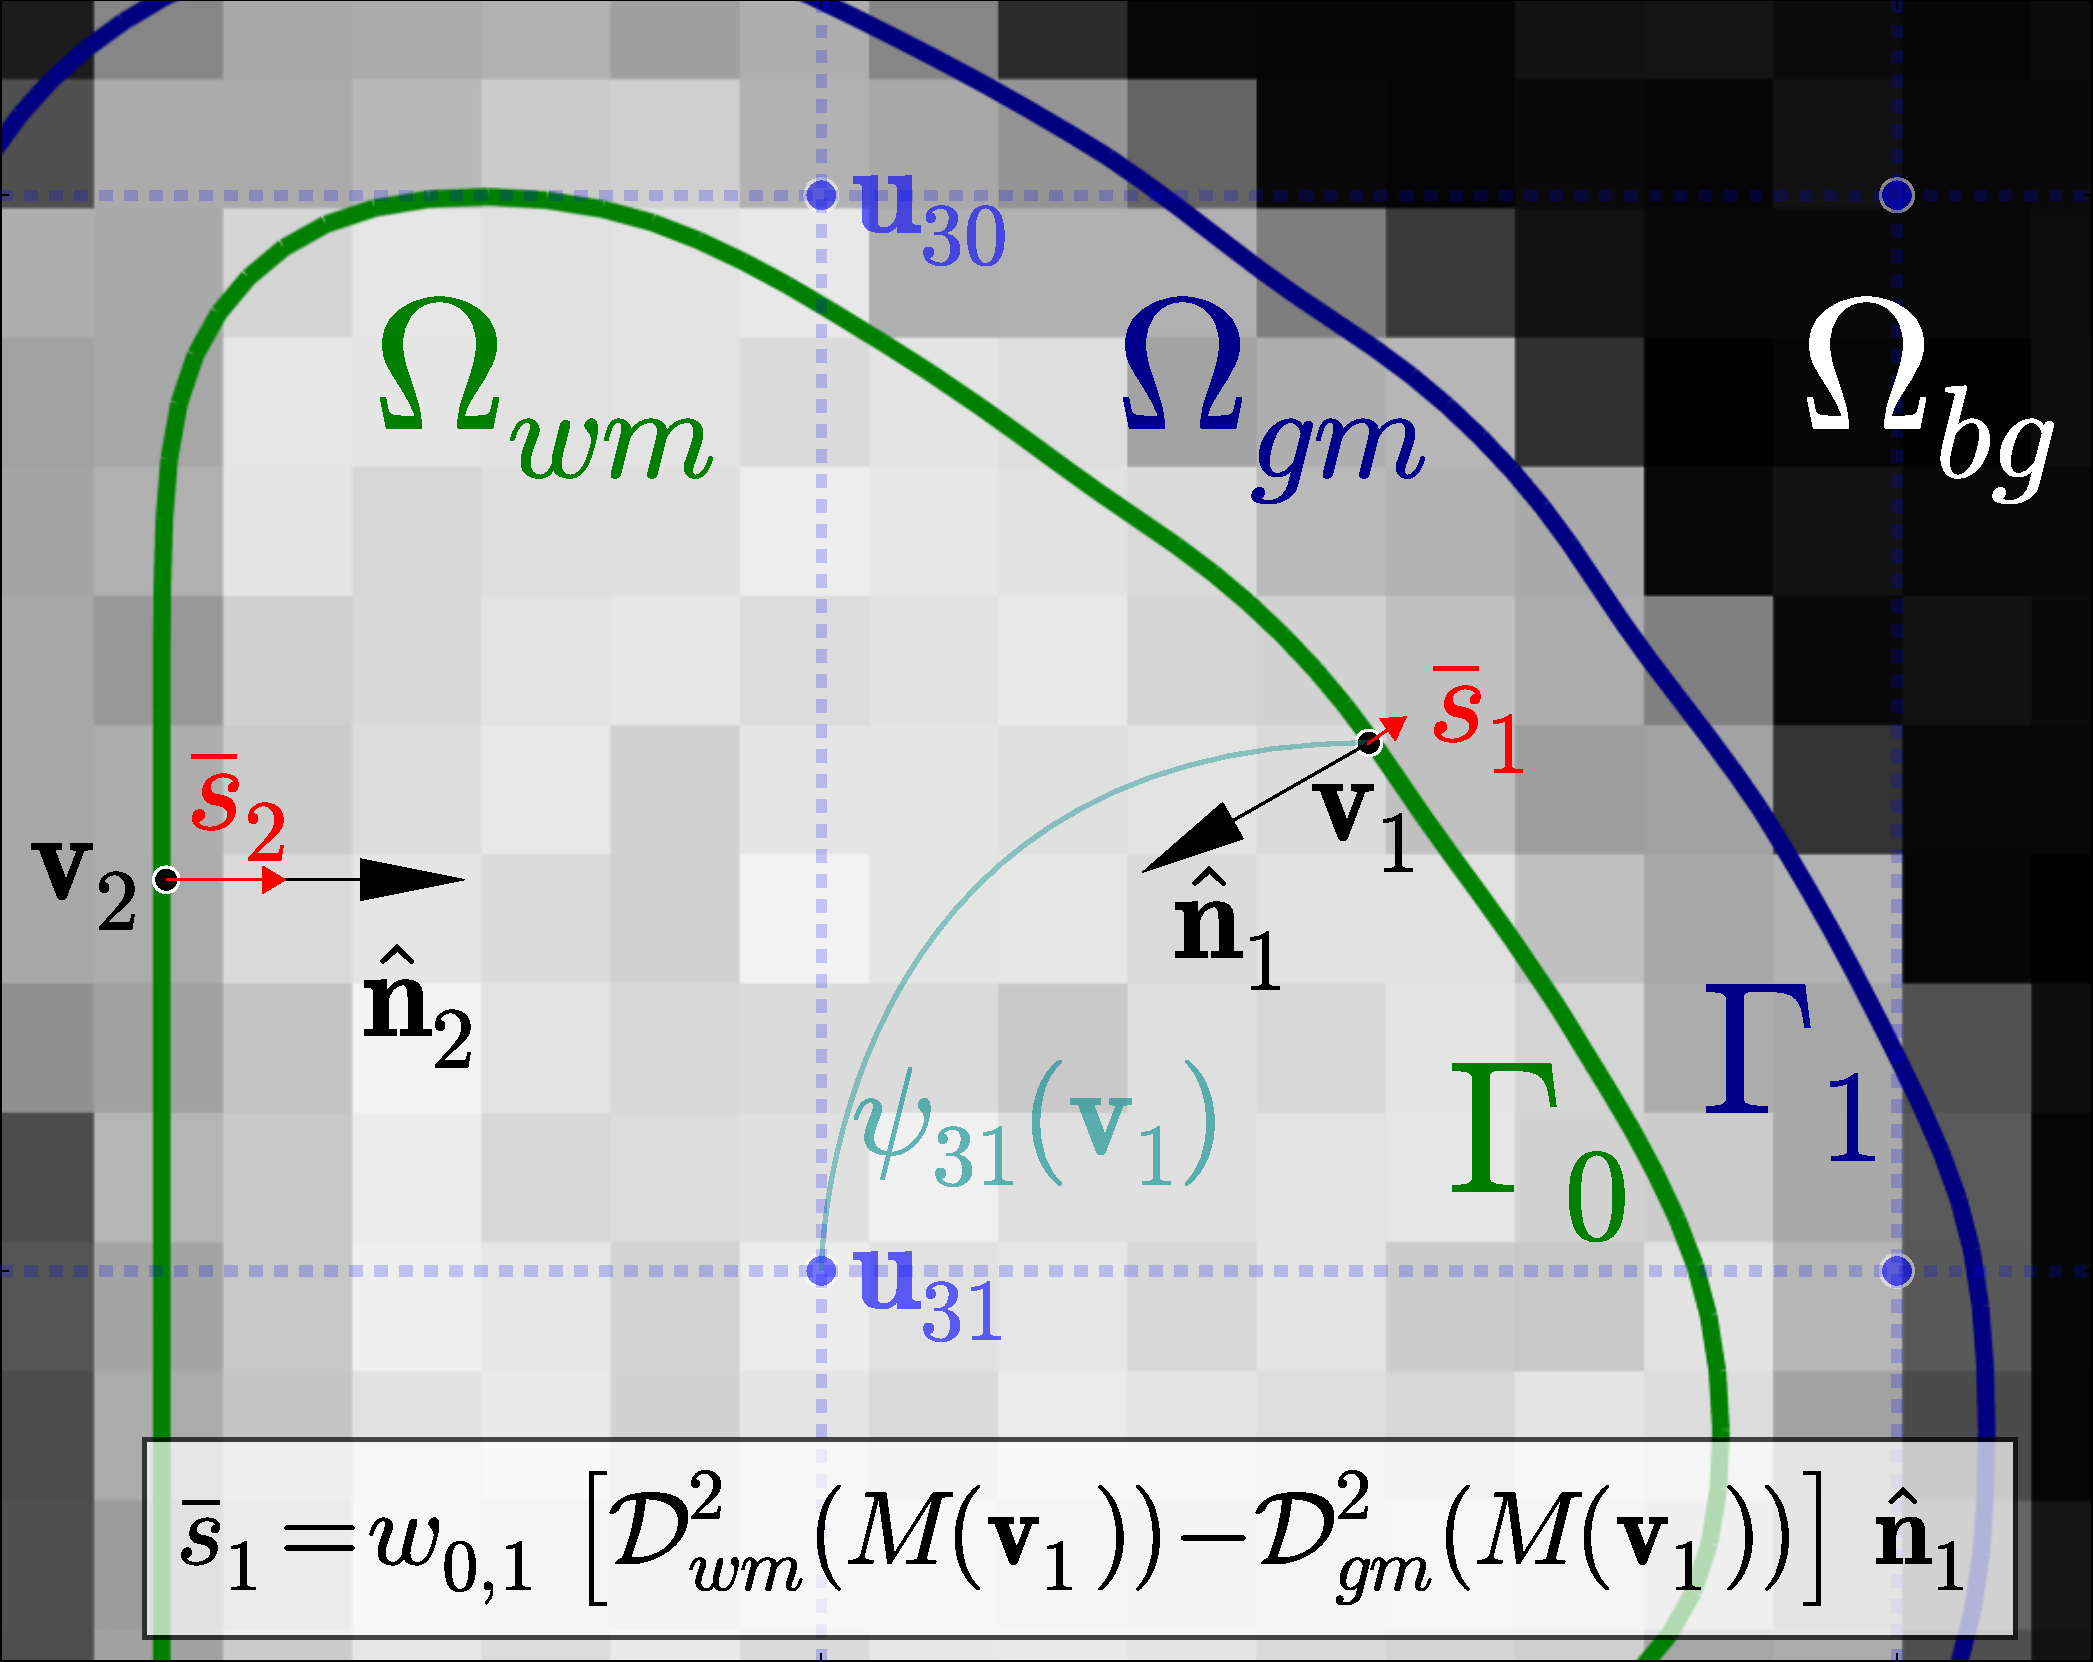
\includegraphics[width=\linewidth]{figure01}
  \caption{The interfacing surfaces $\Gamma_m$ between the competing \glspl{roi} $\Omega_l$,
  play the role of active contours which drive the registration process.
  They evolve iteratively along the normal $\hat{\mathbf{n}}_i$ of the surface at each vertex
    $\vec{v}_i$ of the mesh.
  The gradient speeds $\bar{s}_i$ drive registration, which are computed as the disparity of the data
    energies with respect to the two limiting regions of $M(\vec{v}_i)$, the features of the image
    $M$ in the location of vertex $\vec{v}_i$.
  The computation of shape-gradients is developed in \ref{app:shape_gradients}.
  In this figure, the $\bar{s}_1$ derived from \autoref{eq:regseg-shape_gradient_disc2} is 
    written in the lower box, with $\Omega_{wm}$ being the inner limiting region, $\Omega_{gm}$
    the outer region, and $w_{0,1}$ the relative area associated with vertex $\vec{v}_1$
    with respect to the total area of surface $\Gamma_0$.
  }\label{fig:regseg-method}
\end{figure}

\paragraph*{Cost-function derivation}
In a Bayesian framework for registration \citep{wyatt_map_2003,pohl_bayesian_2006,gass_simultaneous_2014},
  the mappings $U$ in \eqref{eq:regseg-transform} are
  evaluated based on their posterior probability given the observed data
  $M$.
Let $\omegaset = \{\Omega_l: l \in \mathbb{N}, l \leq N_L\}$ be the set of $N_L$ competing regions in
  which $M$ is partitioned by the projection of $\gammaset_R$.
Using Bayes' rule, the posterior likelihood is computed as:

  \begin{equation}
  P(U \mid M, \omegaset ) = \frac{P(M \mid U,\omegaset )\, P(U)}{P(M)},
  \label{eq:regseg-bayes_rule}
  \end{equation}
  where $P(M \mid U,\omegaset)$ is the data likelihood.
Since $\omegaset$ is mapped by $U$, we simplify
  $P(U, \omegaset) = P(U) \implies P(M \mid U,\omegaset) = P(M \mid U)$.
The best estimate $\hat{U}$ then satisfies the maximum a posteriori criterion
  and it aligns $\gammaset_R$ into $M$.
First, we assume independence between \revcomment[R\#3-C10]{voxel}s, and thus we break down the
  global data likelihood into a product of \revcomment[R\#3-C10]{voxel}-wise conditional probabilities:

  \begin{equation}
  P(M \mid U) = \underset{l}{\prod} \underset{\vec{r}'\in \Omega_l}{\prod}
    P\left( \vec{f}' \mid U \right),
  \label{eq:regseg-bayes_aposteriori}
  \end{equation}
  where $\vec{f}' = M(\vec{r}')$ is the feature vector at the displaced
  position $\vec{r}'$ \eqref{eq:regseg-transform} in the moving image.
For convenience and because it has been shown to be an appropriate approximation
  \citep{leemput_automated_1999,cuadra_comparison_2005}, we introduce two assumptions for each
  region $\Omega_l$:
  1) the features are i.i.d.; and 2) they can be modeled by multivariate normal
  distributions 
  $\mathcal{N} (\vec{f}' \mid \boldsymbol{\mu}_l, \boldsymbol{\Sigma}_{l} )$, with parameters
  $\lbrace \boldsymbol{\mu}_l, \boldsymbol{\Sigma}_{l} \rbrace$
  for each region $\Omega_l$ \citep{esteban_mbis_2014}:

  \begin{align}
  P( M \mid U) &= \underset{l}{\prod} \underset{\vec{r}' \in \Omega_l}{\prod}
  \mathcal{N} (\vec{f}' \mid \boldsymbol{\mu}_l, \boldsymbol{\Sigma}_{l} )
  \ifthenelse{\boolean{review}}{=}{= \notag\\ &=}
  \underset{l}{\prod} \underset{\vec{r}' \in \Omega_l}{\prod} \frac{1}{ \sqrt{(2\pi)^{C}\,\left|\boldsymbol{\Sigma}_{l}\right|}}\,{e^{\left(-\frac{1}{2}
  \mdist{f'}{l} \right)}},
  \label{eq:regseg-pdf}
  \end{align}  using $\mdist{f'}{l}$ to denote the squared \emph{Mahalanobis distance} of $\vec{f}'$ with respect
  to the descriptors of region $l$ as
  $\mdist{f'}{l} = (\vec{f}' - \boldsymbol{\mu}_l)^T \, {\boldsymbol{\Sigma}_l}^{-1} \, (\vec{f}' - \boldsymbol{\mu}_l)$.
$C$ is the number of channels comprised in the image $M$.
Even though the features being segmented are not generally i.i.d., the 
  spatial interdependency of voxels is implicitly supported by the piecewise smooth
  partition of the space \omegaset{}.
In fact, the projection of $\gammaset_R$ onto $M$ is an implicit segmentation model, for which
  the covariance matrix $\boldsymbol{\Sigma}_l$ of each region is minimized.
The \autoref{fig:regseg-model} shows how the joint distribution of 
  the input images is approximated with a mixture of multivariate normal distributions,
  and this minimization is illustrated for the segmentation of the \gls*{fa} and the \gls*{adc} maps
  of one subject.

\begin{figure*}
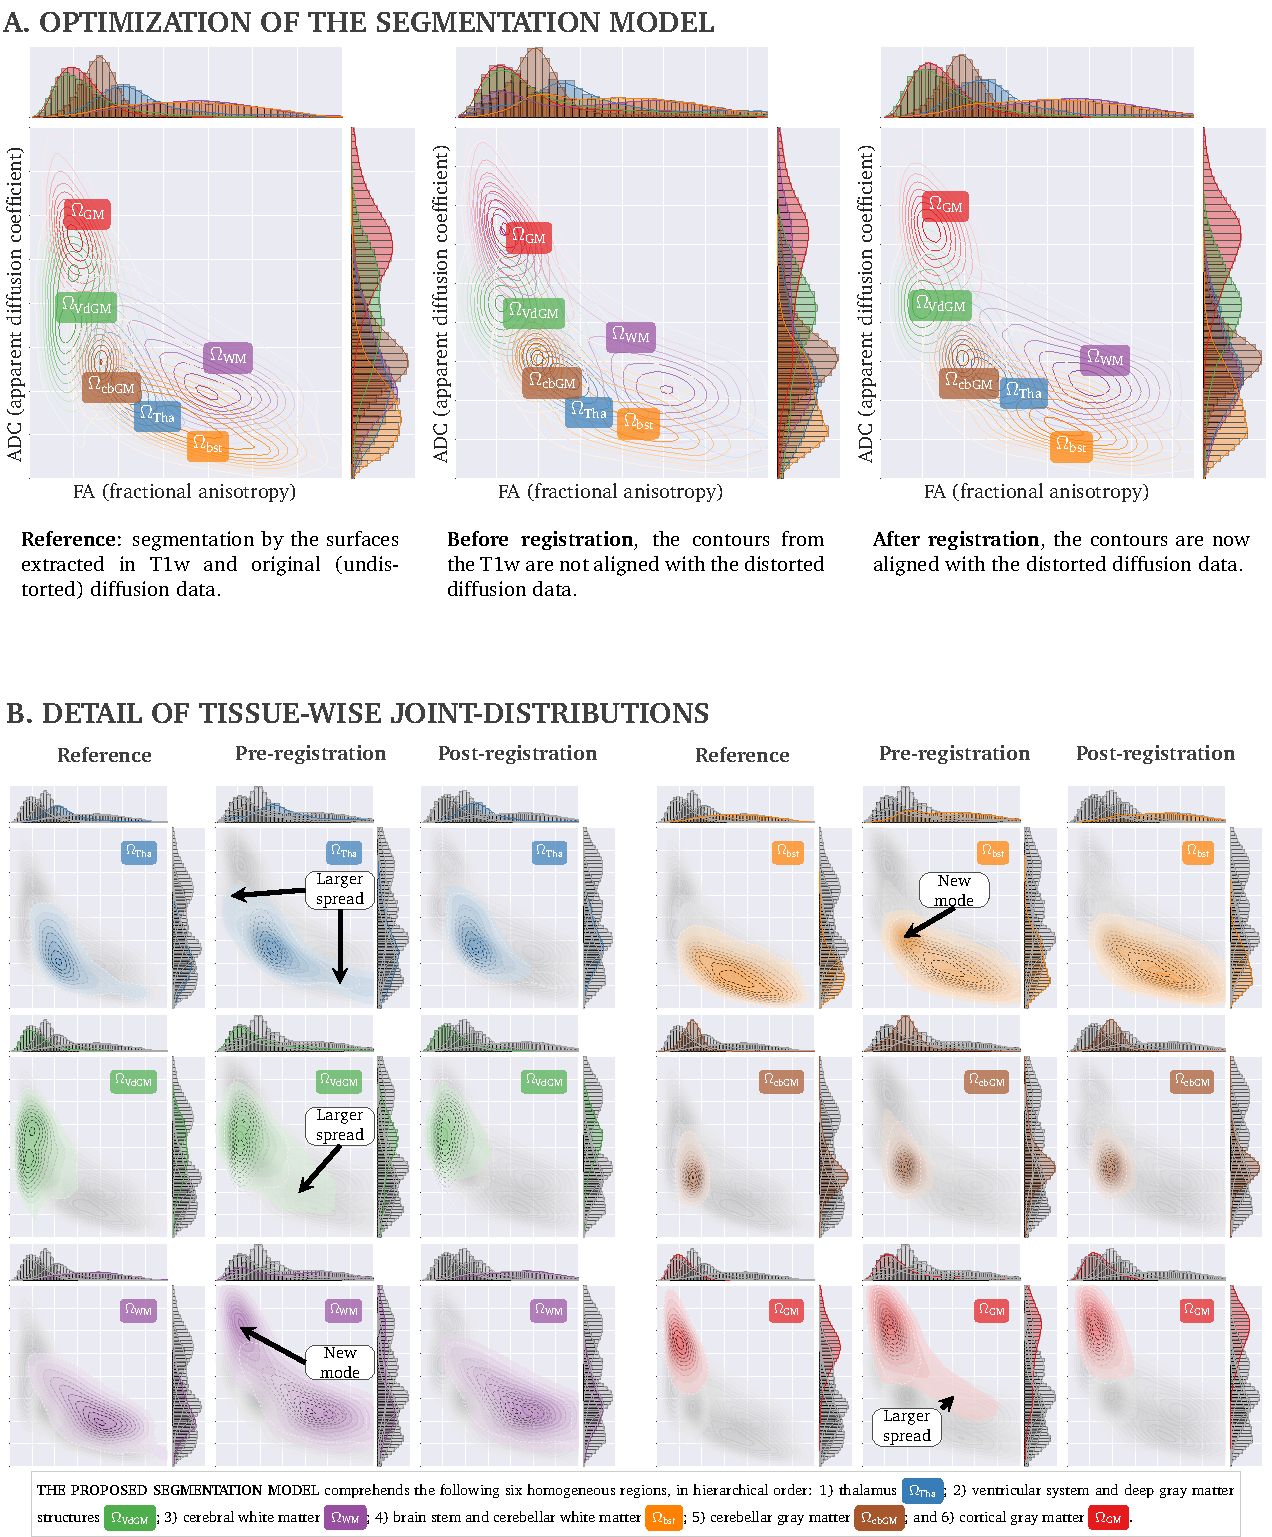
\includegraphics[width=\textwidth]{figure02}
\caption{Evolution of the segmentation model defined by the homogeneous regions $\Omega_l$,
  for one real dataset.
Panel (A, left) shows the joint distribution of the \gls*{fa} and \gls*{adc} conditioned to
  the segmentation \omegaset{} defined by the surfaces $\gammaset_R$ extracted from
  the \gls*{t1} image.
The plot was generated for reference using undistorted diffusion data, and
  therefore, $\gammaset_R$ is aligned with the \gls*{fa} and the \gls*{adc}.
The problem arises when the diffusion data present deformation, and the
  contours $\gammaset_R$ do not fit within the data (A, center).
After registration with \regseg{}, the contours are mapped onto the
  diffusion data (A, right), and the joint density plot is closer to the reference
  situation.
In panel (B), the three plots in (A) are decomposed tissue-wise.
Using filled contours, the bivariate distribution of each tissue is highlighted in its designated color,
  and represented over the remaining tissues (in gray colors).
To help assessment, dashed contours in black-to-white colors represent
  the corresponding distribution in the reference plot.
The registration process optimizes the segmentation model of \regseg{},
  and thus, the distribution of each region after registration is located
  closer to that corresponding in the reference situation, the shape of the distribution
  is more similar to the reference, and their spread is also reduced.
The effects of optimization are more noticeable on the \gls*{gm} ($\Omega_\text{GM}$) and
  the \gls*{wm} ($\Omega_\text{WM}$).
Particularly, the \gls*{wm} typically shows a bimodal distribution when the contours
  \gammaset{} do not fit the data.
{\color{revcolor} The plots in (A) and (B) are provided at full-size in the
  \citetalias[figures S8, S9]{esteban_useful_2016}.}
}\label{fig:regseg-model}
\end{figure*}

\paragraph*{Regularization}
The smoothness of the resulting displacement field is induced
  by a Thikonov regularization prior:

  \begin{align}
  P(U) = \underset{\vec{r}}{\prod}\, p(\vec{u}) &=
  \underset{\vec{r}}{\prod}\, p_0(\vec{u}) \, p_1(\vec{u}), \text{ with} \\
  p_0(\vec{u}) &= \mathcal{N}( \vec{u} \mid 0, \mathbf{A}^{-1}), \notag\\
  p_1(\vec{u}) &= \mathcal{N}(  \nabla \vec{u} \mid 0, \mathbf{B}^{-1}),
  \label{eq:regseg-thikonov}
  \end{align}
 which requires that the distortion and its gradient have zero mean,
   and variance governed by the matrices $\mathbf{A}$ and $\mathbf{B}$.
Therefore, $\mathbf{A}$ and $\mathbf{B}$ are tensors that modulate the regularization, and
  produce deformations with preferential directions.
Finally, the maximum a posteriori problem is adapted to a variational problem where we search for
  the minimum of an energy functional by applying $E(\vec{u}) = -\log \{P( M \mid U) \, P(U)\}$:

  \begin{align}
  E(\vec{u}) &= -\log \underset{l}{\prod}
  \underset{\vec{r}' \in \Omega_l}{\prod}
  \mathcal{N} \left( \vec{f}' \mid \boldsymbol{\mu}_l, \boldsymbol{\Sigma}_l \right)\,p_0( \vec{u})\,p_1( \vec{u}) =
\notag\\ &= - \underset{l}{\sum} \int_{\Omega_l} \Big\{ \log \left[ \mathcal{N} \left( \vec{f}' \mid \boldsymbol{\mu}_l, \boldsymbol{\Sigma}_l \right) \right] \, + \log \left[ p_0( \vec{u})\,p_1( \vec{u}) \right] \Big\} \, d\vec{r}'
   = \notag\\ &=
  \const + \underset{l}{\sum} \Big\{ \int_{\Omega_l} \mdist{f'}{l} \,d\vec{r} \Big\} \,
  + \int_{\Omega} \frac12 \left[ \vec{u}^T \mathbf{A} \vec{u} + (\nabla \vec{u})^T \mathbf{B} (\nabla \vec{u}) \right] \,d\vec{r}'.
  \label{eq:regseg-energy}
  \end{align}This expression is the dual of the Mumford-Shah functional that corresponds
  to the framework of \acrlong*{acwe} \citep{chan_active_2001}
  with the anisotropic regularization term of \cite{nagel_investigation_1986}.


\subsection{Numerical Implementation}
\label{sec:regseg-numerical_implementation}

\paragraph*{Deformation model}\label{sec:regseg-deformation_model}
Since the vertices of the surfaces $\{\vec{v}_i: \vec{v}_i \subset \gammaset \}_{i=1 \ldots N_V}$
  are probably located off-grid, it is necessary to derive $\vec{u}_i = \vec{u}(\vec{v}_i)$ from a discrete set of parameters
  $\{\vec{u}_k\}_{k=1 \ldots K}$.
Densification is achieved using a set of associated basis functions $\psi_k$ \eqref{eq:regseg-nodes_tfm}.
In our implementation, $\psi_k$ is a tensor-product B-spline kernel of degree three.

  \begin{equation}
  \vec{v}_i' = \vec{v}_i + \vec{u}_i = \vec{v}_i + \sum_k \psi_k(\vec{r}) \: \vec{u}_k.
  \label{eq:regseg-nodes_tfm}
  \end{equation}


\paragraph*{Optimization}
\label{sec:regseg-gradient_descent}
To find the minimum of the energy functional \eqref{eq:regseg-energy},
  we propose a gradient-descent approach with respect to the underlying
  deformation field using the following \gls*{pde}:

  \begin{equation}
  \frac{\partial \vec{u}(\vec{r},t)}{\partial t} \propto - \frac{\partial E(\vec{u})}{\partial \vec{u}_k},
  \label{eq:regseg-general_gradient_descent}
  \end{equation}
  where $t$ is an artificial time parameter of the contour
  evolution and $\vec{u}_k$ are the parameters that support the estimate
  $\hat{U}$ of the transformation at the current time point.
Let us assume that the preferential directions of
  the displacement are aligned with the imaging axes to simplify \eqref{eq:regseg-energy} as expression 
  \eqref{eq:regseg-app_energy} in \ref{app:reg_term}, and thus to compute its
  derivative \eqref{eq:regseg-general_gradient_descent}:

  \begin{align}
  \frac{\partial E(\vec{u})}{\partial \vec{u}_k} &=
  \frac{ \partial }{\partial \vec{u}_k} \Big\{
  \underset{l}{\sum} \big[ \int_{\Omega_l} \mdist{f'}{l} \,d\vec{r}' \big] \,
  + \int_{\Omega} \frac12 [ \boldsymbol{\alpha} \cdot \vec{u}^{\circ2}
  + \boldsymbol{\beta} \cdot (\nabla \vec{u})^{\circ2} ] \,d\vec{r}'
  \Big\},
  \label{eq:regseg-gradient_descent}
  \end{align}
  where $\vec{u}^{\circ2} = \vec{u}^T \cdot \vec{u}$,
  and $\{\boldsymbol{\alpha}, \boldsymbol{\beta}\}$ are the expected variances along
  the imaging axes of the displacement field and its gradient, respectively.
Then, the data and regularization terms are split and discretized to compute their
  derivatives.
The derivative of the data term is computed using explicit shape gradients (see \ref{app:shape_gradients}),
  which finally lead to obtain vertex-wise speeds of the gradient $\bar{s}_i$ as
  illustrated in \autoref{fig:regseg-method}.
\revcomment[R\#1-C4]{The shape gradient contributions $\vec{g}_k$ on the field coefficients $\vec{u}_k$
  can then be computed }using the expression \eqref{eq:regseg-gradient_wshape}
\revcomment[R\#1-C4]{of \ref{app:shape_gradients}, obtaining:

\begin{equation}
  \vec{g}_k = - \underset{i}{\sum} \bar{s}_i \cdot \psi_k(\vec{v}_i) \, \hat{\vec{e}}.
  \label{eq:regseg-shape_gradient_final}
\end{equation}

Then,} introducing the analytical derivative of the regularization term,
  the \autoref{eq:regseg-gradient_descent} is reformulated as:

  \begin{align}
  \frac{\partial E(\vec{u})}{\partial \vec{u}_k} &=
  \vec{g}_k  + \boldsymbol{\alpha} \cdot \vec{u}_k - \boldsymbol{\beta} \cdot (\Delta \vec{u}_k).
  \label{eq:regseg-final_gradient}
  \end{align}
Finally, to descend this gradient, we establish a semi-implicit Euler scheme
  \citepalias[see][section S1.3]{esteban_useful_2016},
  with a step size parameter $\delta$, which we solve in the spectral domain as follows:

  \begin{align}
  \vec{u}_k^{t+1} = \mathcal{F}^{-1}\left\{ \frac{\mathcal{F}\{\delta^{-1} \, \vec{u}_k^t - \vec{g}_k\} }
                    {\mathcal{F}\{(\delta^{-1} + \boldsymbol{\alpha})\, I - \boldsymbol{\beta}\Delta\}} \right\},
  \label{eq:regseg-update_equation}
  \end{align}
  where $I$ denotes the identity operator.


\paragraph*{Implementation details and convergence}\label{sec:regseg-conv_report}
The \regseg{} tool includes a multiresolution strategy on the free-form deformation field.
Registration pyramids are created by setting the spacing between the control points of the B-spline basis
  functions for each level of the multiresolution strategy.
As a rule of thumb, for a $\delta =$ 1.0, both $\boldsymbol{\alpha}$
  and $\boldsymbol{\beta}$ will typically be in the range [0.0, 1.0].
The parameters used ($\delta$, $\boldsymbol{\alpha}$, $\boldsymbol{\beta}$, the B-spline grid resolutions,
  and target image smoothing), the implementation details, and other features such as the sparse matrix
  approach to fast interpolation are discussed in the \citetalias[][section S1]{esteban_useful_2016}.

\subsection{Evaluation protocol}\label{sec:regseg-evaluation_protocol}
In order to assess the performance of \regseg{}, we defined the following general
  evaluation protocol:
1) Extract the set of undistorted surfaces $\gammaset_R$;
2) Compute a ground-truth field of displacements $U_\text{true}$, which is applied to
  generate warped images ($M$) for segmentation;
3) Execute \regseg{} with $\gammaset_R$ and use the warped data as inputs; and
4) Perform a visual assessment and compute the error metrics.

A first proof of concept is introduced to demonstrate \regseg{} in digital phantoms
  with simple geometries, using $U_\text{true}$ without directional restrictions.
Then, \regseg{} is evaluated in a framework using undistorted \gls*{dmri} datasets,
  and $U_\text{true}$ is derived from the corresponding inhomogeneity fieldmap of
  the subject.
Therefore, the deformation field is nonzero only in the \acrfull*{pe} axis,
  and reproduces a real \gls*{epi} distortion.
The adaptation of the evaluation protocol to the simulated phantoms and the real data is
  explained in the following sections.

\subsection{Simulated phantoms}\label{sec:regseg-digital_phantoms}
The workflow required to simulate the digital phantoms and to assess the performance of
  \regseg{} with them is presented in \autoref{fig:regseg-evphantoms}.
A set of four binary objects (i.e. ``box'', ``ball'', ``L'',
  and ``gyrus'') was generated by combining the binarization of
  analytical shapes and mathematical morphology.
The reference surfaces $\gammaset_R$ were extracted from the binary shapes
  using \emph{FreeSurfer} tools \citep{fischl_freesurfer_2012}.
The ground-truth distortion was generated using a chain of two displacement
  fields supported by grids of B-spline basis functions.
The coefficients of the basis functions were generated randomly for
  both levels in their three dimensions.
The three components of the displacements $\vec{u} = (u_d)$
  were bounded above by 40\% of the separation between the control points
  at each level to obtain diffeomorphic transforms
  after concatenation \citep{rueckert_diffeomorphic_2006}.
The first deformation field was applied to generate large warpings
  with control points separated by 50.50 mm in the three dimensions
  ($u_d\leq$ 20.20 mm).
With the second warping, we aimed to obtain a field with smoothness
  close to that found in a typical distortion field of \gls*{dmri} data
  \citep{irfanoglu_susceptibility_2011}.
Therefore, the control points were separated by 25.25 mm ($u_d\leq$ 10.10 mm).
After generating the ground-truth deformation, the original surfaces
  were warped by interpolating the displacement field at each vertex.
The warped surfaces $\gammaset_\text{true}$ were binarized to generate tissue fractions
  at low (\isores[mm]{2.0}) and high (\isores[mm]{1.0}) resolutions.
Using an \acrshort*{mri} simulator \citep{caruyer_phantomas_2014}, we synthesized
  \gls*{t1} (TE/TR= 10/1500 ms) and \gls*{t2} images (TE/TR= 90/5000 ms), which
  corresponded to each phantom type, with each at two resolutions
  (1.0 mm and 2.0 mm isotropic).
The field of view at both resolutions was \isores[mm]{100}.
Next, \regseg{} was applied to map $\gammaset_R$ onto the warped phantoms to
  obtain the registered surfaces ($\hat{\gammaset}_\text{test}$).
To quantify the misregistration error, we computed the Hausdorff distance between
 $\hat{\gammaset}_\text{test}$ and $\gammaset_\text{true}$ using \citep{commandeur_vtk_2011}.
In total, 1200 experiments (four phantom types $\times$ 150 random warpings $\times$ two resolutions) were
  performed according to the workflow illustrated in \autoref{fig:regseg-evphantoms}.

\begin{figure*}
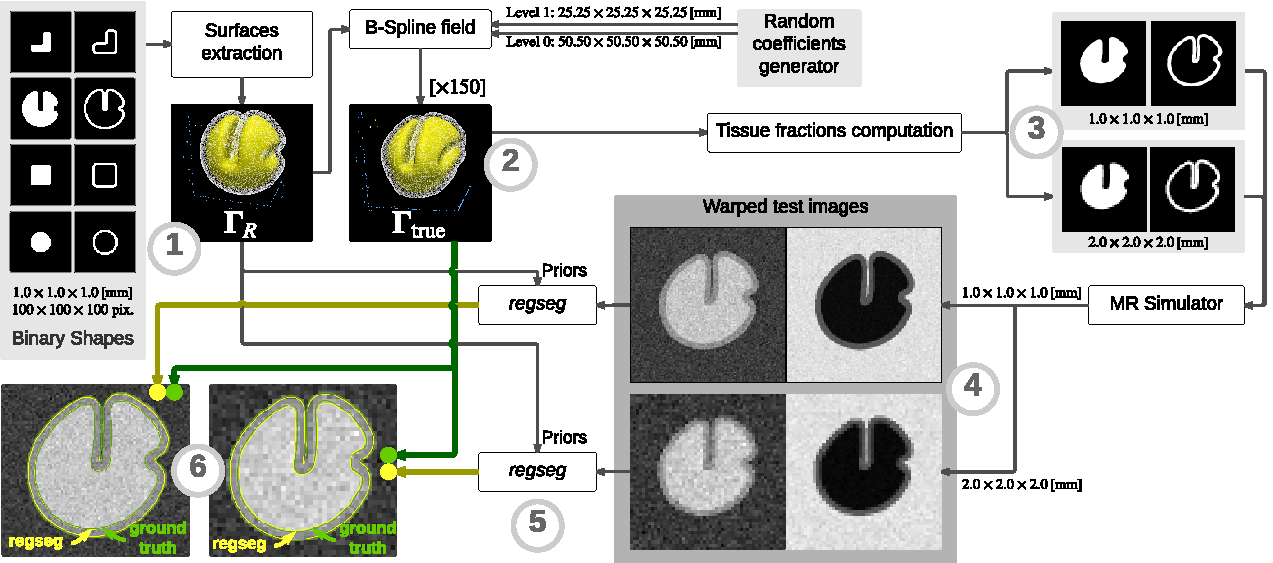
\includegraphics[width=\linewidth]{figure03}
\caption{Evaluation of \regseg{} using phantom data according to the following instrumental workflow.
  1) The reference surfaces $\gammaset_R$ are triangle meshes extracted from the four binary shapes (i.e., ``box'', ``ball'', ``L'', ``gyrus'').
  2) A ground-truth displacement field was generated as described in \autoref{sec:regseg-digital_phantoms}, and applied to warp
      $\gammaset_R$, thereby obtaining $\gammaset_\text{true}$.
  3) After being warped, $\gammaset_\text{true}$ were projected onto the corresponding discrete 3D volume and downsampled to create partial volume effects at two resolutions,
     i.e., \isores[mm]{2.0} and \isores[mm]{1.0}, thereby producing sets of tissue fractions maps.
  4) The tissue fractions were fed into an \acrshort*{mri} simulator, which generated \acrfull*{t1} and \acrfull*{t2} -like images at the
     two possible resolutions.
  5) The \regseg{} tool was applied using the warped test images as multispectral moving images and $\gammaset_R$ as shape priors.
  6) The agreement between the surfaces fitted by \regseg{} ($\hat{\gammaset}_\text{test}$) and $\gammaset_\text{true}$ were assessed
     visually using automatically generated visual reports and quantitatively with the Hausdorff distance between the
     corresponding surfaces.}\label{fig:regseg-evphantoms}
\end{figure*}

\paragraph*{Segmentation model and settings}
The segmentation model of the phantoms is implicitly defined:
  all phantoms comprehend an inner surface enclosing a uniform \gls*{wm}-like region,
  and an outer surface wrapping a \gls*{gm}-like layer.
The outside is filled with uniform background (see \autoref{fig:regseg-evphantoms}).
All the experimental settings used for the phantoms are made available in
  a unique configuration file\footnote{\url{https://github.com/oesteban/RegSeg/blob/master/Scripts/pyacwereg/data/regseg_default.json}}.

\subsection{Real datasets} \label{sec:regseg-human_connectome}
The experimental framework for the real datasets is presented in \autoref{fig:regseg-evworkflows},
which extends our previous evaluation \citep{esteban_simulationbased_2014} of distortions
  using \gls*{dmri} phantoms.

\begin{figure*}
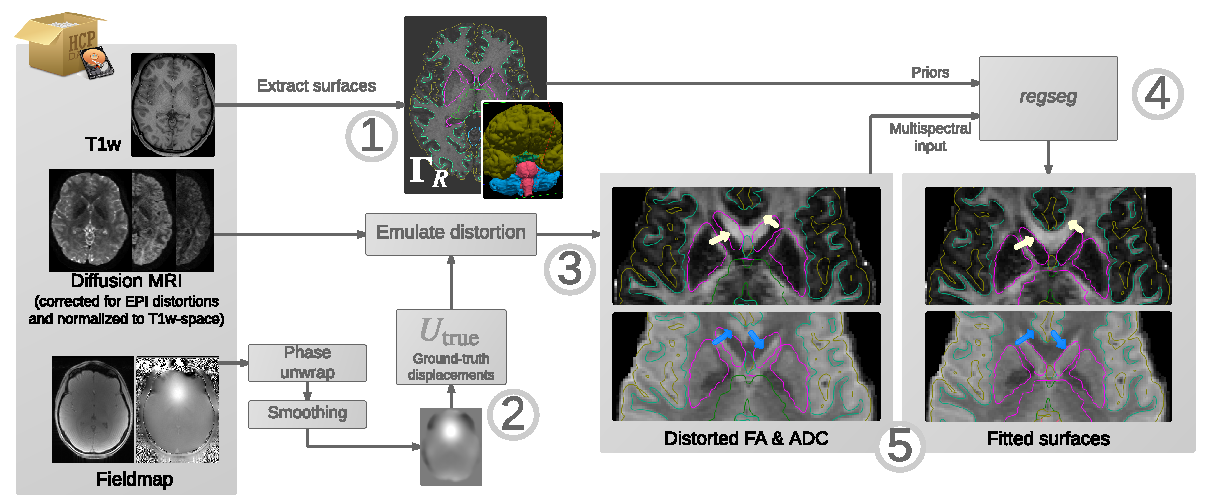
\includegraphics[width=\linewidth]{figure04}
\caption{Experimental workflow employed to process real data from the \acrfull*{hcp}.
  1) $\gammaset_R$ were extracted from the anatomical reference (\gls*{t1} image).
  2) For use as the ground truth, we generated a plausible synthetic distortion $U_\text{true}$
    from the fieldmap with \eqref{eq:regseg-fieldmap}.
  3) The \gls*{dmri} data were warped using $U_\text{true}$ to reproduce the effects of real
    susceptibility-derived distortions.
  Target diffusion scalars (\gls*{fa} and \gls*{adc}) were computed with the distorted data and
    stacked to feed the multivariate input required by \regseg{}.
  4) The method was run to obtain $U_\text{test} = \hat{U}_\text{true}$, i.e., the estimate of
    the ground-truth deformation.
  5) The results were evaluated visually and quantitatively.
  The arrows in the step (5) point to edges in the target images (light-yellow arrows for \gls*{fa}, blue for 
    \gls*{adc}) that should be aligned with a surface, showing how distortion limits the direct mapping from
    the structural space in which the contours are defined.}\label{fig:regseg-evworkflows}
\end{figure*}


\paragraph*{Data}
To evaluate \regseg{} using real \gls*{dmri} data obtained from human brains,
  we collected 16 subjects from the \revcomment[R\#3-C9]{Q3 Release of the}
  \gls*{hcp} database.
The original acquisitions are released within ``unprocessed'' packages, whereas
  the ``minimally preprocessed'' packages contain the corresponding images after
  some processing (correction for several artifacts, brain-extraction, spatial
  normalization, etc.).
We refer the reader to \citet{essen_human_2012} for exact details of the acquisition
  parameters and \citet{glasser_minimal_2013} for the preprocessing issues.
These datasets comprise a large set of images, including \gls*{t1}, \gls*{t2}, and
  multi-shell \gls*{dmri} images.
Since we obtained the \gls*{dmri} data from the minimally preprocessed package, these
  images are corrected for \gls*{epi} distortions and spatially normalized in
  \gls*{t1} space.
\revcomment[R\#3-C9]{In the Q3 Release of the \gls*{hcp}, the \gls*{dmri} session includes
  six runs, two runs for each of three different gradient tables, and each table is acquired
  once with right-to-left and left-to-right encoding polarities, respectively.
Then, the diffusion datasets with opposed polarities are corrected for susceptibility
  distortions using the \emph{TOPUP} tool \citep{andersson_how_2003}
  before producing the released ``minimally preprocessed'' data}.

\paragraph*{Segmentation model}
Based on our experience   and previous studies \citep{ennis_orthogonal_2006},
  we defined the moving image as a stack of the \gls*{fa} and \gls*{adc} maps derived
  from \gls*{dmri} data.
After evaluating several alternative models, we empirically defined a partition \omegaset{}
  according to the following six regions:
  1) thalamus ($\Omega_\text{Tha}$);
  2) ventricular system and deep \gls*{gm} structures ($\Omega_\text{VdGM}$);
  3) cerebral \gls*{wm} ($\Omega_\text{WM}$);
  4) brain stem and cerebellar \gls*{wm} ($\Omega_\text{bst}$);
  5) cerebellar \gls*{gm} ($\Omega_\text{cbGM}$); and
  6) cortical \gls*{gm} ($\Omega_\text{GM}$).
Using tools in \emph{FreeSurfer} and appropriate selections of labels in the
  \emph{aparc} segmentation released with the \gls*{hcp} data, we extracted the $\gammaset_R$ set for the
  reference surfaces.
The segmentation model corresponding to this partition is shown in \autoref{fig:regseg-model}
  and discussed in greater detail in the \citetalias[section S4]{esteban_useful_2016}.

\paragraph*{Ground-truth generation}
Realistic deformation was achieved by generating displacement fields that satisfy the theoretical
  properties of distortion.
The displacements along the \gls*{pe} axis of the \gls*{dmri} image are related to the local
  deviation of the field $\Delta B_0(\vec{r})$ from its nominal value $B_0$  \citep{jezzard_correction_1995},
  as follows:

  \begin{equation}
  u_\text{PE} = \frac{\gamma \, T_{acq}\, s_\text{PE}}{2\pi}\Delta B_0(\vec{r})\text{ [mm]},
  \label{eq:regseg-fieldmap}
  \end{equation}
where $\gamma$ is the gyromagnetic ratio, $T_{acq}$ is the readout time, and
  $s_\text{PE}$ is the \revcomment[R\#3-C10]{voxel} size along \gls*{pe}.
Certain \acrshort*{mri} sequences are designed to estimate $\Delta B_0$, thereby obtaining
  the so-called fieldmap.
We derived the deformation $U_\text{true}$ from the fieldmap image released with
  the corresponding packages of each dataset in the \gls*{hcp}.
The fieldmap was unwrapped\footnote{fieldmaps are phase maps, which are intrinsically clipped in the interval
  of $[-\pi, \pi)$ [rads] or [rads/s].} and smoothed before applying \eqref{eq:regseg-fieldmap}.
Next, the original \gls*{dmri} was warped using the resulting displacement field and fed into
  a pipeline to process the corresponding \gls*{dti}, thereby computing the derived scalars of
  interest (\gls*{fa} and \gls*{adc}) using \emph{MRtrix} \citep{tournier_mrtrix_2012}.

\paragraph*{Metric assessment}
Initially, we investigated the appropriateness of the segmentation model.
For five test datasets, we uniformly sampled the space of distortions
  $\hat{U} = \epsilon \cdot U_\text{true} = \vec{r} + \epsilon \, u_\text{PE}$
  (with $\epsilon \in [-1.1, 1.1]$ and $u_\text{PE}$ from \eqref{eq:regseg-fieldmap}),
  and we evaluated the data term of the cost function \eqref{eq:regseg-energy}.
The minimum of the cost function (\autoref{sec:regseg-methods_map}) was consistently located at
  $\epsilon=0.0$ (the ground-truth) for all of the cases \citepalias[figure S2]{esteban_useful_2016}.

\paragraph*{Settings} \Regseg{} accepts an affine mapping from surface-space to the \gls*{dmri} data as initialization.
However, the images provided by the \gls*{hcp} are already spatially normalized.
Therefore, the initial estimation of distortion is zero in this experiment.
Since the distortion $U_\text{true}$ is aligned along the \gls*{pe} direction ($y$-axis in our settings),
  \regseg{} was configured to allow nonzero displacements only on that corresponding direction.
For the experiments on real data, \regseg{} established a multi-resolution pyramid of
  B-spline functions, with control points distributed on grids of the following spacings:
  40$\times$100$\times$40 [mm] for the first (coarser) level, \isores[mm]{30} for the second level,
  and 20$\times$30$\times$10 [mm] in the third level.
Only the first and second levels included Gaussian smoothing of the target image ($\sigma$ = [2.0, 0.5] mm,
  respectively).
The actual choices of the parameter settings are publicly distributed with the source code for the
  experiments\footnote{\url{https://github.com/oesteban/RegSeg/tree/master/Scripts/pyacwereg/data/regseg_hcp.json}}.
These settings were obtained manually, driven by the feedback obtained from the post-registration
  convergence reports \citepalias[like that found in][section S1.3]{esteban_useful_2016}.
We released \regseg{} along with the tool to generate such convergence reports.

\paragraph*{Cross-comparison} A dual workflow to the general evaluation used for \regseg{} (\autoref{fig:regseg-evworkflows}),
  was employed to integrate the alternate \gls*{t2b} registration scheme.
We reproduced the solution and settings provided with \emph{ExploreDTI}
  \citep{leemans_exploredti_2009}, which is a widely used toolkit for tractography analysis of
  \gls*{dti}.
\emph{ExploreDTI} internally employs \emph{elastix} \citep{klein_elastix_2010} to
  perform registration.
The deformation field is correspondingly restricted to the \gls*{pe} direction.
The settings file for \emph{elastix} is also
  available\footnote{\url{https://github.com/oesteban/RegSeg/blob/master/Scripts/pyacwereg/data/t2b_elastix_y.txt}}.
\revcomment[R\#3-C7\\R\#3-C8]{In this registration scheme, the \gls*{t2} image is the \emph{reference} and
  the \lowb{} plays the role of \emph{moving} image.
Therefore, the transform is defined in the coordinate system of the \gls*{t2} image,
  and for each point in this space it provides the location of the corresponding feature
  in the \lowb{} image.
Since the surfaces are defined in the \gls*{t2} --\emph{reference}-- space, their coordinates
  can be mapped to the \lowb{} space using this transform, obtaining the 
  \emph{distorted surfaces} corresponding to the \lowb{}-to-\gls*{t2} registration.}


\paragraph*{Error measurement}\label{sec:regseg-experiments_evaluation}
Distortion only occurs along the \gls*{pe} axis of the image, so we computed the
  \gls*{swindex} as the area-weighted distance between the corresponding vertices of
  $\gammaset_\text{true}$ and their estimate obtained by the method under the test $\hat{\gammaset}_\text{test}$:

  \begin{equation}
  sWI = \frac{1}{\sum_i a_i} \sum\limits_i^{N_V} a_i\,\|
  \vec{v}_i - \hat{\vec{v}}_i \|,
  \label{eq:regseg-swindex}
  \end{equation}
  where $\vec{v}_i \subset \gammaset_\text{true}$ are the locations of the total $N_V$ vertices,
  $a_i$ is the area corresponding to each vertex $\vec{v}_i$,
  and $\hat{\vec{v}}_i \subset \hat{\gammaset}_\text{test}$ are the recovered locations
  that correspond to $\vec{v}_i$.
In practice, we only report the \gls*{swindex} for three surfaces (\{$\Gamma_\text{VdGM}, \Gamma_\text{WM}, \Gamma_\text{pial}$\})
  of crucial interest in whole-brain tractography.
\revcomment[R\#3-C7\\R\#3-C8]{The \gls*{swindex} is always computed on the \gls*{dmri} space.}   \section{Results}
\label{sec:regseg-results}

\subsection{Verification and validation using digital phantoms}
\label{sec:regseg-results_phantom}

The results summarized in \autoref{fig:regseg-phantom} demonstrated that the accuracy was
  high and below the image resolution.
Panel B on \autoref{fig:regseg-phantom} shows the violin plots for each model type corresponding
  to the two sets of resolutions for the generated phantoms.
In order to relate the average misregistration error to the resolution of the moving image,
  we proceeded as follows.
First, we confirmed that the vertex-wise error distributions were skewed by using Shapiro-Wilk's test of
  normality.
All of the distributions of errors in the tests (four phantom types $\times$ two resolutions) were
  nonnormal with $p<$ 0.001.
Consequently, we used the nonparametric Wilcoxon signed-rank test with the Bonferroni
  correction for multiple comparisons ($N$=150, for each phantom type).
The average errors were significantly lower than the voxel size with $p <$ (0.001 / 150)
  in all tests (four phantom types $\times$ two resolutions).
Statistical tests might not be sufficiently conclusive, so we also computed the confidence intervals,
  as shown in \autoref{tab:ci_phantom}.

\begin{figure*}[!h]
  \centering
  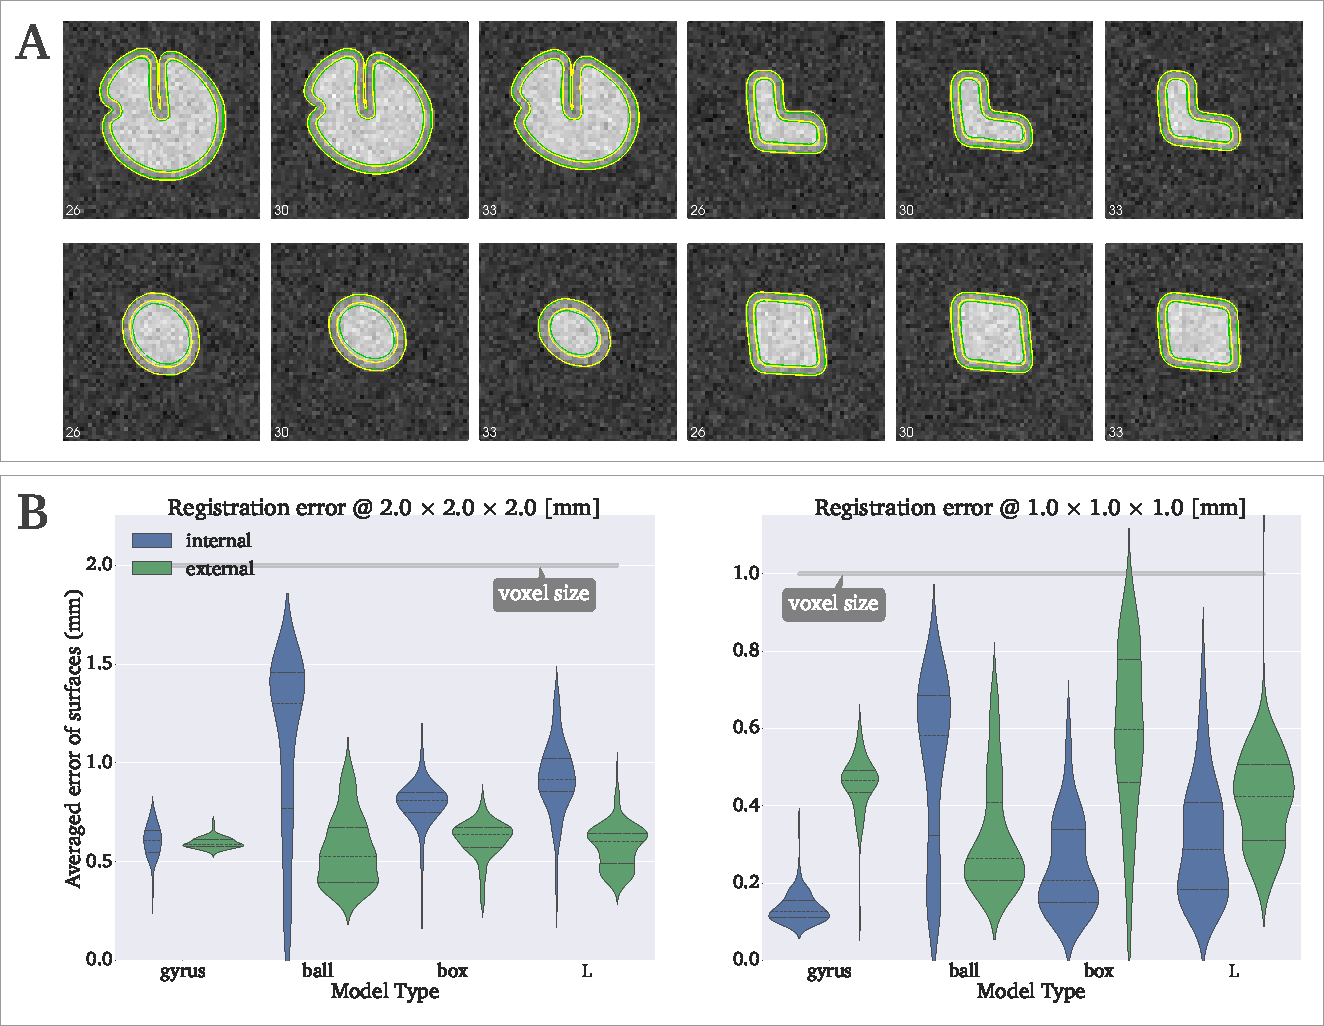
\includegraphics[width=\linewidth]{figure05}
  \caption{A. Visual assessment of the results obtained on the digital phantoms.
    The panel shows three coronal slices (indices indicated on the lower left corner) of each phantom
    volume at low resolution:
    ``gyrus'' (top left), ``L'' (top right), ``ball'' (bottom left),
    and ``box'' at (bottom right).
  The contours recovered after registration are represented in yellow.
  \Regseg{} achieved high accuracy because it determined the almost exact locations of the registered
    contours with respect to their ground truth positions (shown in green).
  The partial volume effect makes segmentation of the sulci a challenging problem with voxel-wise
    clustering methods, but they were successfully segmented with \regseg{}.
  B. Quantitative evaluation: the violin plot shows the variability across experiments
    of the average Hausdorff distance measured in each vertex of the corresponding surface, for the
    low (left) and high (right) resolutions. 
    Error averages were consistently below the size of the voxel.
    }\label{fig:regseg-phantom}
\end{figure*}
\begin{figure*}[!h]
  \centering
  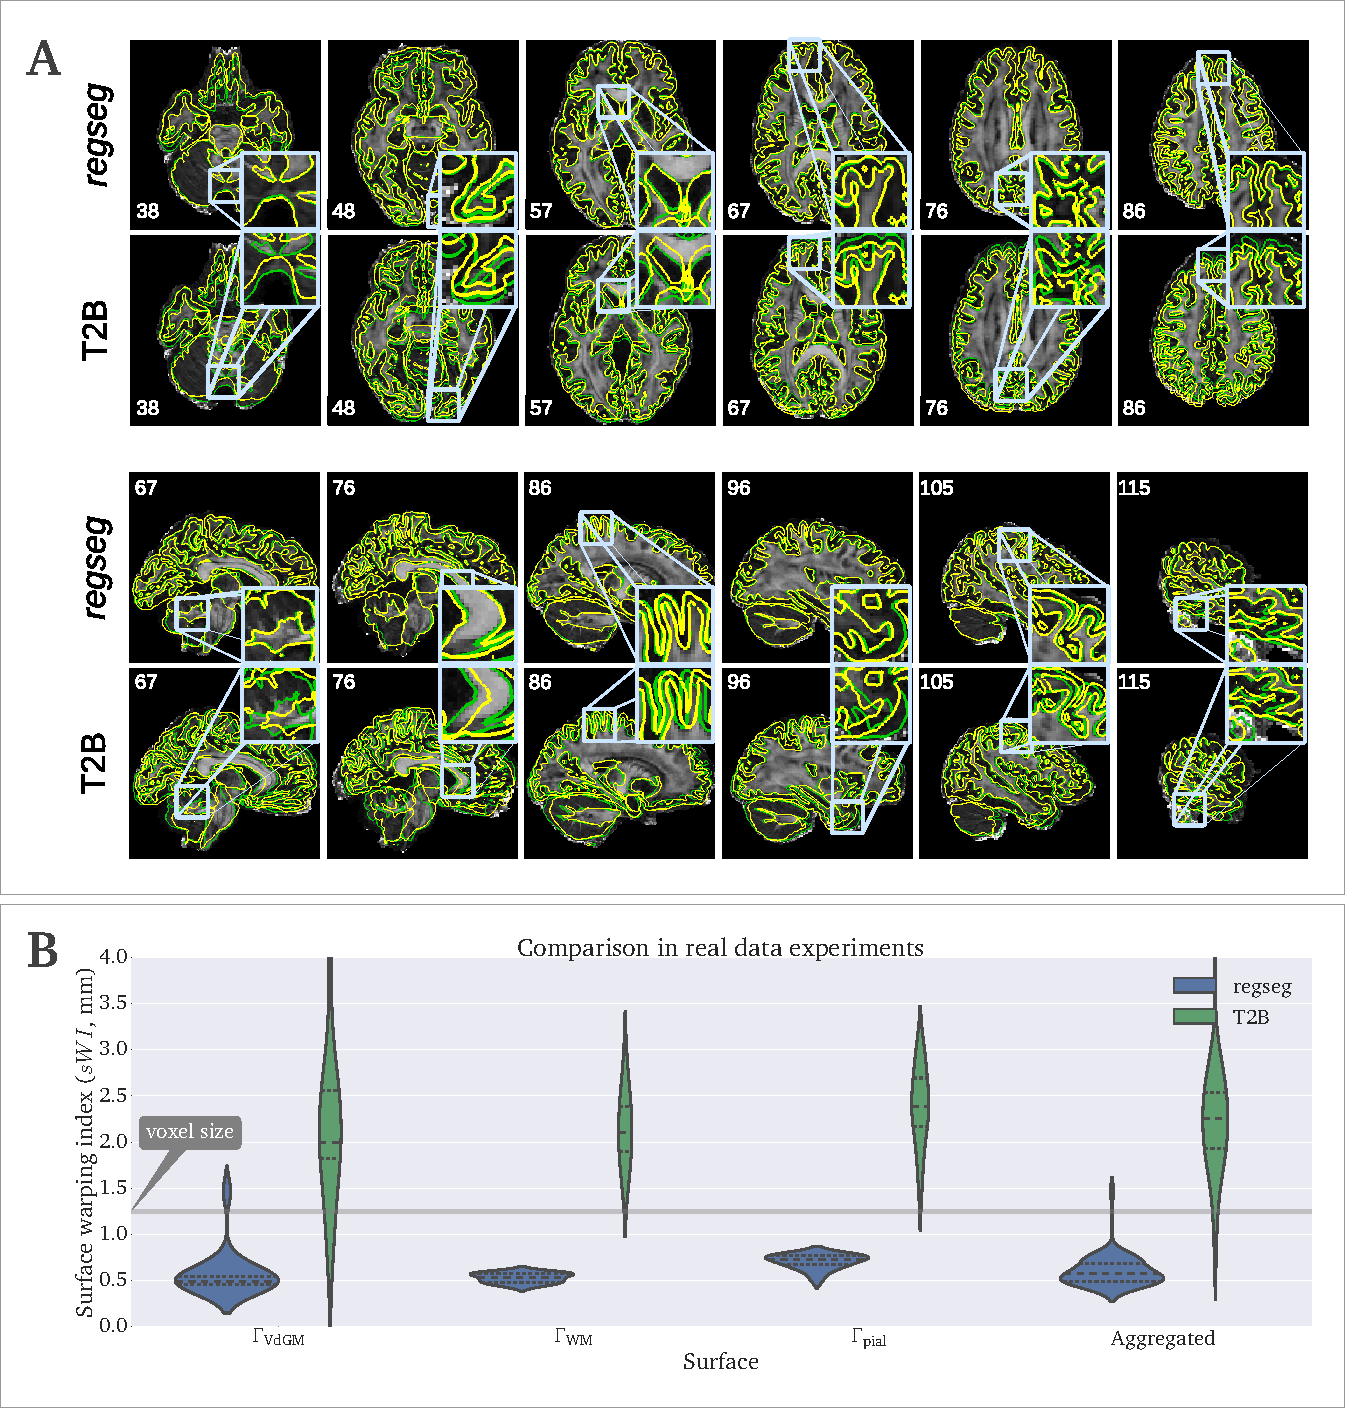
\includegraphics[width=\linewidth]{figure06}
  \caption{A. Example of a visual assessment report, which was automatically generated by the evaluation tool.
    Each view shows one component of the input image (in this case, the \gls*{fa} map), the ground-truth locations
    of the surfaces (green contours), and the resulting surfaces obtained with the test method (yellow contours).
  The first two rows show axial slices for \regseg{} and the \acrfull*{t2b} method, while the last two rows
    show the corresponding sagittal views.
  The coronal view is omitted because it was the least informative due to the directional property
    of the distortions.
  Specific regions where \regseg{} outperformed \gls*{t2b} are enlarged.
  B. Violin plots of the error distributions for each surface across the 16 subjects, which show the 
    voxel size of the \gls*{dmri} images (1.25 mm), thereby supporting the improved results obtained
    by \regseg{} with the proposed settings.
  }\label{fig:regseg-results_real}
\end{figure*}

\subsection{Evaluation using real datasets and cross-comparison}\label{sec:regseg-results_hcp}
Finally, we compared the performance of \regseg{} with that of the standard \gls*{t2b}
  method.
Summary reports for visual assessment of the 16 cases are included in the
  \citetalias[section S5]{esteban_useful_2016}.
In \autoref{fig:regseg-results_real}, box A, the visual report is shown for one subject.
We computed the \gls*{swindex} \eqref{eq:regseg-swindex} of every surface after registration
  using both the \regseg{} and \gls*{t2b} methods.
Finally, to compare the results, we performed Kruskal-Wallis H-tests
  (a nonparametric alternative to ANOVA) on the warping indices for the three surfaces of
  interest selected in \autoref{sec:regseg-experiments_evaluation}
  ($\Gamma_\text{VdGM}$, $\Gamma_\text{WM}$, $\Gamma_\text{pial}$).
All of the statistical tests showed that the error distributions obtained with \regseg{} and
  \gls*{t2b} were significantly different, and the violin plots in box B of
  \autoref{fig:regseg-results_real} demonstrate that the errors were always larger with \gls*{t2b}.
We also show the 95\% CIs of the \gls*{swindex} for these surfaces 
  (\autoref{tab:results_real}).
The aggregate CI for \regseg{} was 0.56--0.66 [mm], whereas the \gls*{t2b} method
  yielded an aggregate CI of 2.05--2.39 [mm].
The results of the statistical tests and the CIs are summarized in \autoref{tab:results_real}.

\begin{table}
\centering
\footnotesize
\tabcolsep=0.1cm
\begin{minipage}{.48\textwidth}
    \vskip-4.7ex
    \begin{tabular}{lccccc}
    Res.   & ``gyrus'' & ``ball''  & ``box''   & ``L''     & Aggreg.    \\\hline
    1.0mm  & 0.18--0.38 & 0.31--0.45 & 0.34--0.42 & 0.34--0.40 & 0.34--0.38  \\
    2.0mm  & 0.59--0.60 & 0.65--0.76 & 0.68--0.71 & 0.67--0.77 & 0.64--0.66  \\
    \hline
    \end{tabular}
    \caption{The distributions of vertex-wise Hausdorff distances between the ground-truth surfaces and their
    corresponding estimates obtained with \regseg{} presented a 95\% CI below the half-voxel size for all of
    the phantom types.
    The CIs were computed by bootstrapping using 10$^\text{4}$ samples, with the median as the location statistic.}\label{tab:ci_phantom}
\end{minipage}
\hfill
\begin{minipage}{.48\textwidth}
    \begin{tabular}{cccccc}
    & & $\Gamma_\text{VdGM}$  & $\Gamma_\text{WM}$ & $\Gamma_\text{pial}$ & Aggreg. \\
    \hline
    \multirow{2}{*}{CI}
       & \regseg{} & 0.50--0.78 & 0.50--0.55 & 0.66--0.73 & 0.56--0.66 \\
       & T2B       & 1.78--2.58 & 1.94--2.36 & 2.16--2.58 & 2.05--2.39 \\
    \hline
    \multirow{2}{*}{H-tests}
       & p-value  & 4.1\e{-6} & 2.3\e{-6} & 2.3\e{-6} & 1.8\e{-16} \\
       & H-stat   & 21.20 & 22.31 & 22.31 & 67.85 \\
    \hline
    \end{tabular}
    \caption{Statistical analysis of results obtained using 16 real datasets from 
    the \gls*{hcp}, which show that \regseg{} performed better than the alternative \acrfull{t2b} method.
    The distribution of the errors computed for the surfaces of interest ($\Gamma_\text{VdGM}$, $\Gamma_\text{WM}$, $\Gamma_\text{pial}$)
      and the aggregate of all surfaces (Aggreg. column) had lower 95\% CIs with \regseg{}.
   The CIs in this table were computed by bootstrapping using the mean as the location statistic and with 10$^\text{4}$ samples.
    The Kruskal-Wallis H-tests indicated that there was a significant difference between the results obtained using \regseg{} and
      the \gls*{t2b} method.
    }\label{tab:results_real}
\end{minipage}
\end{table} \section{Discussion}
\label{sec:regseg-discussion}
We present \regseg{}, a simultaneous segmentation and registration method that
  maps a set of nested surfaces into a multivariate target-image.
The nonlinear registration process evolves driven by the fitness of the
  piecewise-smooth classification of voxels in the target volume imposed
  by the current mapping of the surfaces.
We propose \regseg{} to map anatomical information extracted from \gls*{t1}
  images into the corresponding \gls*{dmri} of the same subject.
Previously, joint segmentation and registration has been applied successfully to
  other problems such as longitudinal object tracking \citep{paragios_level_2003}
  and atlas-based segmentation \citep{gorthi_active_2011}.
The most common approach involves optimizing a deformation model (registration)
  that supports the evolution of the active contours (segmentation),
  like \cite{paragios_level_2003,yezzi_variational_2003}.
\Regseg{} can be seen as a particular case of atlas-based segmentation-registration methods,
  replacing the atlas by the structural image of the subject (\emph{structure-informed segmentation}).
The main difference of atlas-based segmentation and the application at hand is the resolution of the
  target image.
Atlas-based segmentation is typically applied on structural and high-resolution images.
A comprehensive review of joint segmentation and registration methods applied in atlas-based
  segmentation is found in \citep{gorthi_active_2011}.
They also propose a multiphase level-set function initialized from a labeled atlas to implement
  the active contours that drive the atlas registration.
Alternatively, \regseg{} implements the active contours with a hierarchical set of explicit
  surfaces (triangular meshes) instead of the multiphase level sets, and registration
  is driven by shape-gradients \citep{herbulot_segmentation_2006}.
As an advantage, the use of explicit surfaces enables segmenting \gls*{dmri} images
  with accuracy below \revcomment[R\#3-C10]{voxel} size.

An important antecedent of \regseg{} is \emph{bbregister} \citep{greve_accurate_2009}.
The tool has been widely adopted as the standard registration method to be used along with the \gls*{epi}
  correction of choice.
It implements a linear mapping and uses 3D active contours \emph{with edges} to
  search for intensity boundaries in the \lowb{} image.
The active contours are initialized using surfaces extracted from the \gls*{t1} using
  \emph{FreeSurfer} \citep{fischl_freesurfer_2012}.
To overcome the problem of nonlinear distortions, \emph{bbregister} excludes from the
  boundary search those regions that are typically warped.
Indeed, the distortion must be addressed separately because it is not supported by
  the affine transformation model.
Conversely, the deformation model of \regseg{} is nonlinear and the active contours are
  \emph{without edges} \citep{chan_active_2001} since the \gls*{fa} and \gls*{adc} maps
  do not present steep image gradients (edges) but the anatomy can be identified
  by looking for piece-wise smooth homogeneous regions.

Recently, \cite{guyader_combined_2011} proposed a simultaneous segmentation and
  registration method in 2D using level sets and a nonlinear elasticity smoother on the
  displacement vector field, which preserves the topology even with very large deformations.
\Regseg{} includes an anisotropic regularizer for the displacement field described by
  \cite{nagel_investigation_1986}.
This regularization strategy conceptually falls in the midway between the Gaussian smoothing
  generally included in most of the existing methodologies, and the complexity of
  the elasticity smoother of \cite{guyader_combined_2011}.
Other minor features that differ from current methods in joint segmentation and registration are
  the support of multivariate target-images and the efficient computation of the shape-gradients
  implemented with sparse matrices.

We verified that precise segmentation and registration of a set of surfaces into multivariate
  data is possible on digital phantoms.
We randomly deformed four different phantom models to mimic three homogeneous regions
  (\gls*{wm}, \gls*{gm}, and \acrlong*{csf}) and we used them to simulate \gls*{t1}
  and \gls*{t2} images at two resolution levels.
We measured the Hausdorff distance between the contours projected using the
  ground-truth warping and the estimations found with \regseg{}.
We concluded that the errors were significantly lower than the voxel size.
We also assessed the 95\% \gls*{ci}, which yielded an aggregate interval of
  0.64--0.66 [mm] for the low resolution phantoms (2.0 mm isotropic voxel) and
  0.34--0.38 [mm] for the high resolution phantoms (1.0 mm isotropic).
Therefore, the error was bounded above by half of the voxel size.
The distributions of errors along surfaces varied importantly depending on the shape of the
  phantom (see \autoref{fig:regseg-phantom}B).
The misregistration error of the ``gyrus'' phantom showed a much lower spread than that
  for the other shapes.
We argue that the symmetry of those other shapes posed difficulties in driving the contours
  towards the appropriate region due to \emph{sliding} displacements between the
  surfaces and their ground-truth position.
The effect is not detectable by the active contours framework, but it is controllable
  increasing the regularization constraints.
When \regseg{} is applied on real datasets, this surface sliding is negligible for the
  convoluted nature of cortical surfaces and the directional restriction of the
  distortion.

We evaluated \regseg{} in a real environment using the experimental framework presented
  in \autoref{fig:regseg-evworkflows}.
We processed 16 subjects from the \gls*{hcp} database using both \regseg{}
  and an in-house replication of the \acrfull*{t2b} method.
\Regseg{} obtained a high accuracy, with an aggregate 95\% \gls*{ci} of 0.56--0.66 [mm], which was
  below the \revcomment[R\#3-C10]{voxel} size of 1.25 mm.
The misregistration error that remained after \regseg{} was significantly lower ($p <$ 0.01) than the
  error corresponding to the \gls*{t2b} method according to Kruskal-Wallis H-tests
  (\autoref{tab:results_real}).
Visual inspections of all the results \citepalias[section S5]{esteban_useful_2016} and the violin plots in
  \autoref{fig:regseg-results_real} confirmed that \regseg{} achieved higher accuracy
  than the \gls*{t2b} method in our settings.
We carefully configured the \gls*{t2b} method using the same algorithm and the
  same settings employed in a widely-used tool for \gls*{dmri} processing.
However, cross-comparison experiments are prone to the so-called \emph{instrumentation bias}
  \citep{tustison_instrumentation_2013}.
Therefore, these results did not prove that \regseg{} \emph{is better than} \gls*{t2b},
  but indicated that \regseg{} is a reliable option in this application field.
Finally, we also proposed a piecewise-smooth segmentation model defined by
  a selection of nested surfaces to partition the multispectral space
  comprehending the \gls*{fa} and the \gls*{adc} maps and ultimately identify anatomical
  structures in \gls*{dmri} space.
We also demonstrated the smoothness of the objective function on five of the real datasets
  \citepalias[figure S2]{esteban_useful_2016}, taking advantage of the directional
  restriction of possible distortions.
However, \regseg{} requires densely sampled surfaces to ensure the convergence.
Using the digital phantoms, we severely decimated the surfaces by a large factor.
These surfaces introduced a bias which displaced the zero of the gradients from the
  minimum of the objective function impeding the convergence.

The proposed application of the method in the task of identifying structural information
  in \gls*{dmri} images is an active field of research \citep{jeurissen_tissuetype_2015}.
Current processing of \gls{dmri} involved in the connectome extraction and other applications
  (such as \gls*{tbss} or surgical planning) require a precise segmentation
  of the anatomical structures in the diffusion space.
Some examples of these processing tasks are the structure-informed reconstruction of \gls*{dmri}
  data \citep{jeurissen_multitissue_2014,daducci_accelerated_2015}, the anatomically constrained
  tractography \citep{smith_anatomicallyconstrained_2012}, and the imposition of the cortical
  parcellation mapped from the \gls*{t1} image \citep{hagmann_mapping_2008}.
The problem was firstly addressed using image segmentation approaches in the native diffusion
  space, without definite and compelling results.
With the introduction of retrospective correction methods for the \emph{\gls*{epi} distortions}
  and image registration approaches, the task has been typically solved in a two-step approach.
First, the \glspl*{dwi} are corrected for \emph{\gls*{epi} distortions} by estimating
  the nonlinear deformation field from extra MR acquisitions
  \citep{jezzard_correction_1995,chiou_simple_2000,cordes_geometric_2000,kybic_unwarping_2000}.
Second, mapping the structural information from the corresponding \gls*{t1} image
  using a linear registration tool like \emph{bbregister} \citep{greve_accurate_2009}.
The current activity on improving correction methods \citep{irfanoglu_drbuddi_2015} and
  the comeback of segmentation of \gls*{dmri} in its native space
  \citep{jeurissen_tissuetype_2015} proof the open interest of this application.
\Regseg{} addresses this joint problem in a single step and it does not require any additional
  acquisition other than the minimal protocol comprehending only \gls*{t1} and \gls*{dmri} images.
This situation is commonly found in historical datasets.

We envision \regseg{} to be integrated in diffusion processing pipelines, after a 
  \revcomment[R\#3-C10]{preliminary}
  \gls*{dti} computation and before anatomically-informed reconstruction and tractography
  methods.
Since the structural information is projected into the native space of \gls*{dmri},
  these two processes and the matrix building task can be performed on the unaltered
  \gls*{dmri} signal (i.e. without resampling data to an undistorted space).
For analyses other than connectivity, like \gls*{tbss}, the deformation estimated by \regseg{}
  can be used to map the tracts into structural space.
\revcomment[R\#3-C5]{Even though we apply \regseg{} to the problem of susceptibility distortion,
  \emph{it is not a distortion correction method}, but rather a surface alignment method.
In fact, the distortions are not corrected in the \gls*{epi} data.}
\revcomment[R\#3-C6]{Therefore, we suggest here to perform the reconstruction and tractography processes in the
  original (distorted) diffusion data.}
\revcomment[R\#1-C3]{\Regseg{} allows to avoid resampling and/or unwarping of the diffusion signal because the 
  structural information necessary in the diffusion analysis is mapped from the
  reference space.}
\revcomment[R\#1-C1]{Certain applications (like \gls*{tbss}) and methodologies (like building the connectivity matrix
  by clustering the tracks) may not be performed correctly on the native (distorted) diffusion space
  because they still need a mapping to the undistorted space.
Using \regseg{}, the tracks obtained in native space can be unwarped using the resulting estimation
  of the deformation field.}
\revcomment[R\#3-C6]{This methodological variation will be further investigated, to ensure which processing design
  yields the most accurate tractography results.}

Beyond the presented application on \gls*{dmri} data, \regseg{} can be indicated in situations
  where there are precise surfaces delineating the structure, a target multivariate
  image in which the surfaces must be fitted, and the mapping between the surfaces and
  the volume encodes relevant physiological information, such as the normal/abnormal
  development or the macroscopic dynamics of organs and tissues.
For instance, \regseg{} may be applied in fields like neonatal brain image segmentation
  in longitudinal MRI studies of the early developmental patterns \citep{shi_neonatal_2010}.
In these studies, the surfaces obtained in a mature time point of the brain are retrospectively
  propagated to the initial time points, regardless of the changes in the contrast and spatial
  development between them.
More generally, \regseg{} may also be applied to the personalized study of longitudinal alteration
  of the brain using multispectral images, for instance in the case of traumatic brain
  injury \citep{irimia_structural_2014} or in monitoring brain tumors
  \citep{weizman_semiautomatic_2014}.
 

\section*{Conclusion}
\label{sec:regseg-conclusion}

\Regseg{} is a variational framework for the simultaneous segmentation and
  registration of 3D \gls*{dmri} data obtained from the human brain, where within-subject
  anatomical information is used as a reference.
The registration method segments the target multivariate image into several competing regions, which are
  defined explicitly by their limiting surfaces.
The surfaces are active and they evolve on a free-form deformation field supported by the B-spline basis.
A descent optimization strategy is guided by shape gradients computed on the current partition
  of the target image.
\Regseg{} uses active contours without edges and it searches for
  homogeneous regions within the image.
We tested \regseg{} using digital phantoms by simulating \gls*{t1} and \gls*{t2} \acrshort*{mri}
  warped with smooth and random deformations.
The resulting misregistration of the contours was significantly lower than the image resolution
  of the phantoms.

We proposed \regseg{} for simultaneously segmenting and registering \gls*{dmri} data to
  their corresponding \gls*{t1} image from the same subject.
We demonstrated the accuracy of the proposed method based on visual assessments of the results
  obtained by \regseg{} and cross-comparisons with a widely used technique.
Moreover, \regseg{} does not require any images in addition to the minimal acquisition protocol,
  which only utilizes \gls*{t1} and \gls*{dmri}.
As well as the proposed application to \gls*{dmri} data, other potential uses of \regseg{} are
  atlas-based segmentation and tracking objects in time-series.


\section*{Availability and reproducibility statement}
\label{sec:regseg-availability}
We considered the reproducibility of our results as a design requirement.
Therefore, we used real data obtained from the Human Connectome Project \citep{essen_human_2012}
  and all of the software utilized in this study is also publicly available.
\Regseg{} was implemented on top of ITK-4.6 (Insight Registration and
  Segmentation Toolkit, \url{http://www.itk.org}).
The evaluation instruments (\autoref{fig:regseg-evworkflows}) were implemented using
  \emph{nipype} \citep{gorgolewski_nipype_2011} to assess their reproducibility.
All of the research elements (data, source code, figures, manuscript sources, etc.) involved in this study
  are publicly available under a unique package \citep{esteban_regseg_2015}.
 
\section*{Author contributions}
All the authors contributed to this study.
OE implemented the method, designed and conducted the experiments, wrote the paper,
  simulated the phantoms, and prepared the real data.
DZ devised and drafted the registration method, generated early phantom datasets, and
  collaborated in the implementation of the method.
AD, MBC, and MJLC interpreted the results.
AD, MBC, MJLC, JPT, and AS advised on all aspects of the study.

\section*{Acknowledgments}
The authors thank Y. Alem\'an and G. Wollny for their thorough reviews of the manuscript,
  V. Estellers for early discussions at the beginning of this project,
  and L. A. Vese for her support during OE's research visits to her laboratory.
We also thank A. Leemans for kindly sharing a p-code version of \emph{ExploreDTI} from
  which the settings for \emph{elastix} could be extracted.

DZ was supported by the Swiss National Science Foundation under grants PBELP2-137727, 
  P300P2-147778, and NSF-DMS 1418812.
This study was supported by the Spanish Ministry of Science and Innovation
  (projects TEC-2013-48251-C2-2-R and INNPACTO XIORT), Comunidad de Madrid (TOPUS) and
  European Regional Development Funds, the Center for Biomedical Imaging
  (CIBM) of the Geneva and Lausanne Universities and the EPFL, as well as the
  Leenaards and Louis Jeantet Foundations. 

\onecolumn
\appendix
\numberwithin{equation}{section}

\renewcommand{\theequation}{A.\arabic{equation}}
\renewcommand{\thesubsection}{Appendix \arabic{subsection}}

\section*{Appendix}

\subsection{Simplifying the regularization term}\label{app:reg_term}
The exponentials of the Thikonov regularization prior \eqref{eq:regseg-thikonov} have the general form
  $\vec{v}^T \mathbf{M} \vec{v}$.
If $\mathbf{M}$ is a $n \times n$ diagonal matrix such that $\mathbf{M} = \vec{m} \, \mathbf{I}_n$,
  then:

\begin{equation*}
\vec{v}^T \mathbf{M} \vec{v} = \vec{m} \cdot (\vec{v}^T \mathbf{I}_n \vec{v}) = \vec{m} \cdot \vec{v}^{\circ2},
\end{equation*}
  where we have introduced the Hadamard power notation\footnote{The Hadamard power of a matrix or a vector
  is the power of its elements $\mathbf{M}^{\circ p} = ({m_{ij}}^{p})$}.

In general, the anisotropy of the distortion field is aligned with the 
  voxel coordinate system, so
  $\mathbf{A}$ and $\mathbf{B}$ of \eqref{eq:regseg-energy} can be simplified to diagonal matrices
  to regularize the registration process, such that
  $\mathbf{A}= \, \boldsymbol{\alpha}\,\vec{I}_n$ and
  $\mathbf{B}= \, \boldsymbol{\beta}\,\vec{I}_n$.
By substituting into equation \eqref{eq:regseg-energy}, we obtain:

  \begin{align}
  E(\vec{u}) &= \const + \, \underset{l}{\sum} \int_{\Omega_l} \mdist{f'}{l} \,d\vec{r} \,
  \ifthenelse{\boolean{review}}{+}{+ \notag\\ &+}
  \int_{\Omega} \frac12 \left[ \boldsymbol{\alpha} \cdot \vec{u}^{\circ2} + \boldsymbol{\beta} \cdot (\nabla \vec{u})^{\circ2} \right] \,d\vec{r}.
  \label{eq:regseg-app_energy}
  \end{align}

\subsection{Application of the shape-gradients}\label{app:shape_gradients}
The computation of gradients at the locations of the active contours in the
  instant $t$ is based on the work of \cite{herbulot_segmentation_2006}.
Let $F(\vec{r})$ be an ``arbitrary'' function over the image domain
  $\Omega = \Omega_l \cup \Omega_m$ split in two regions $l$ and
  $m$, and $\Gamma_{l,m}$ a closed boundary between them.
We now derive the domain integral w.r.t. $t$:

  \begin{equation}
  \frac{\partial}{\partial t} \int_\Omega F(\vec{r}) d\vec{r} =
  \int_\Omega \frac{\partial}{\partial t}F(\vec{r}) d\vec{r}
  - \int_{\Gamma_{l,m}} F(\vec{r}) \left\langle \frac{\partial \Gamma_{l,m} }{\partial t},
  N_{\Gamma_{l,m}}\right\rangle d\vec{r},
  \end{equation}
  where $\left\langle\frac{\partial\Gamma_{l,m}}{\partial t}, N_{\Gamma_{l,m}}\right\rangle$ is
  the projection of the boundary movement on the unit inward normal $N_{\Gamma_{l,m}}$.
Assuming that the region descriptors $\{\boldsymbol{\mu}_l, \boldsymbol{\Sigma}_l\}$ vary slowly enough, we can consider
  that $\frac{\partial}{\partial t} F(\vec{r}) = 0$ and thus:

  \begin{equation}
  \frac{\partial}{\partial t} \int_\Omega F(\vec{r}) d\vec{r} =
  - \int_{\Gamma_{l,m}} F(\vec{r}) \left\langle \frac{\partial \Gamma_{l,m} }{\partial t},
  N_{\Gamma_{l,m}}\right\rangle d\vec{r}.
  \label{eq:regseg-shape_gradients}
  \end{equation}

The equation \eqref{eq:regseg-shape_gradients} is discretized as follows.
First, the surface between limiting regions $l$ and $m$ ($\Gamma_{l,m}$) is explicitly represented by
  a discrete set of vertices $\vec{v}_i$, with $i \in \{0, \ldots, N_p -1 \}$.
Consequently, the inwards normal of the surface $N_{\Gamma_{l,m}}$ is represented by the discrete
  set of normals $\hat{\vec{n}}_i$ at each vertex of the mesh.
The resulting summation is, therefore, discrete and the integral operator is replaced by the sum:

  \begin{align}
  \frac{\partial}{\partial t} \int_\Omega F(\vec{r}) d\vec{r} &=
  \underbracket{\cancel{\int_\Omega \frac{\partial}{\partial t}F(\vec{r}) d\vec{r} }}_{\text{Functional's evolution}}
  - \underbracket{\int_{\Gamma_{l,m}} F(\vec{r}) \left\langle \frac{\partial \Gamma_{l,m}}{\partial t},
  N_{\Gamma_{l,m}}\right\rangle d\vec{r}}_{\text{Shape's evolution}} \notag \\
  & = - \underset{p}{\sum} \frac{1}{A_p} \underset{i}{\sum} \, a_i \, F(\vec{v}_i) \left\langle \underbracket{\frac{\partial \vec{v}_i}{\partial t}}_{\text{speed of }\vec{v}_i},
  \hat{\vec{n}}_{i}\right\rangle.
  \label{eq:regseg-shape_gradient_orig}
  \end{align}
where $a_i$ is the area corresponding to vertex $\vec{v}_i$, and $A_p = \sum_i a_i$ is the total area of the surface $p$.
In the following, we will refer as $w_{p,i} = a_i / A_p $ to the area contribution of $\vec{v}_i$ to the
  total area of the surface it belongs to.
For simplicity, the sum over $p$ can be also removed, as the vertices belong to only one of the total $P$ contours.

Then, the speed of $\vec{v}_i$ is discretized using the artificial time-step parameter $\delta$, as the displacement
  $\frac{\partial \vec{v}_i}{\partial t} = \vec{v}_i(\delta = t+1) - \vec{v}_i(\delta = t)$:

  \begin{equation}
  \frac{\partial}{\partial t} \int_\Omega F(\vec{r}) \, d\vec{r} =
  - \underset{i}{\sum} w_{p,i} F(\vec{v}_i) \frac{\partial \vec{v}_i}{\partial t} \cdot \hat{\vec{n}}_i.
  \label{eq:regseg-shape_gradient_disc1}
  \end{equation}

Since the energy functional is defined over competing regions, the displacement of $\vec{v}_i$ will cause
  an energy exchange between the limiting regions, and therefore $F(\vec{r})$ must be split in
  two terms, $F_{in}(\vec{r})$ corresponding to the interior region and $F_{out}(\vec{r})$ to the exterior:

  \begin{equation}
  \frac{\partial}{\partial t} \int_\Omega F(\vec{r}) \, d\vec{r} =
  - \underset{i}{\sum} \, \frac{\partial \vec{v}_i}{\partial t} \cdot
  \underbracket{w_{p,i} \, \Big[ F_{out}(\vec{v}_i) - F_{in}(\vec{v}_i) \Big] \hat{\vec{n}}_i}_{\bar{s}_i \text{ in Figure 1}}.
  \label{eq:regseg-shape_gradient_disc2}
  \end{equation}

Then, we identify the shape gradient contribution $\vec{g}_k$ on the coefficients $\vec{u}_k$ of the B-spline grid 
\revcomment[R\#1-C4]{to obtain the definition of $\vec{g}_k$ given in \eqref{eq:regseg-final_gradient}}:

  \begin{equation}
  \label{eq:regseg-gradient_wshape}
  \begin{split}
  \vec{g}_k &= - \underset{i}{\sum} \left\langle \frac{\partial \vec{v}_i'}{\partial \vec{u}_k}, \bar{s}_i'\right\rangle \\
  \text{with }
  \bar{s}_i' &= w_i \left[ \mdist{f_i'}{out} - \mdist{f_i'}{in} \right] \, \hat{\vec{n}}_i, \\
  \text{and }
  \frac{\partial \vec{v}_i'}{\partial \vec{u}_k} &=
  \frac{\partial}{\partial \vec{u}_k} \left\{ \vec{v}_i + \sum_k \psi_k(\vec{v}_i) \vec{u}_k \right\} = \psi_k(\vec{v}_i)\, \hat{\vec{e}},
  \end{split}
  \end{equation}\revcomment[R\#1-C4]{where $\psi_k$ and $\vec{u}_k$ define our B-spline deformation model (\autoref{eq:regseg-nodes_tfm})} and
  $\hat{\vec{e}}$ is the coordinates system's unit vector.


 \ifthenelse{\boolean{review}}
{}
{\twocolumn}

\bibliographystyle{mystyle}
\bibliography{Remote}


\end{document}
